\documentclass{article}

% packages
  % basic stuff for rendering math
  \usepackage[letterpaper, top=1in, bottom=1in, left=1in, right=1in]{geometry}
  \usepackage[utf8]{inputenc}
  \usepackage[english]{babel}
  \usepackage{amsmath} 
  \usepackage{amssymb}
  % \usepackage{amsthm}

  % extra math symbols and utilities
  \usepackage{mathtools}        % for extra stuff like \coloneqq
  \usepackage{mathrsfs}         % for extra stuff like \mathsrc{}
  \usepackage{centernot}        % for the centernot arrow 
  \usepackage{bm}               % for better boldsymbol/mathbf 
  \usepackage{enumitem}         % better control over enumerate, enumerate
  \usepackage{hyperref}         % for hypertext linking
  \usepackage{fancyvrb}          % for better verbatim environments
  \usepackage{newverbs}         % for texttt{}
  \usepackage{xcolor}           % for colored text 
  \usepackage{listings}         % to include code
  \usepackage{lstautogobble}    % helper package for code
  \usepackage{parcolumns}       % for side by side columns for two column code
  

  % page layout
  \usepackage{fancyhdr}         % for headers and footers 
  \usepackage{lastpage}         % to include last page number in footer 
  \usepackage{parskip}          % for no indentation and space between paragraphs    
  \usepackage[T1]{fontenc}      % to include \textbackslash
  \usepackage{footnote}
  \usepackage{etoolbox}

  % for custom environments
  \usepackage{tcolorbox}        % for better colored boxes in custom environments
  \tcbuselibrary{breakable}     % to allow tcolorboxes to break across pages

  % figures
  \usepackage{pgfplots}
  \pgfplotsset{compat=1.18}
  \usepackage{float}            % for [H] figure placement
  \usepackage{tikz}
  \usepackage{tikz-cd}
  \usepackage{circuitikz}
  \usetikzlibrary{arrows}
  \usetikzlibrary{positioning}
  \usetikzlibrary{calc}
  \usepackage{graphicx}
  \usepackage{caption} 
  \usepackage{subcaption}
  \captionsetup{font=small}

  % for tabular stuff 
  \usepackage{dcolumn}

  \usepackage[nottoc]{tocbibind}
  \pdfsuppresswarningpagegroup=1
  \hfuzz=5.002pt                % ignore overfull hbox badness warnings below this limit

% New and replaced operators
  \DeclareMathOperator{\Tr}{Tr}
  \DeclareMathOperator{\Sym}{Sym}
  \DeclareMathOperator{\Span}{span}
  \DeclareMathOperator{\std}{std}
  \DeclareMathOperator{\Cov}{Cov}
  \DeclareMathOperator{\Var}{Var}
  \DeclareMathOperator{\Corr}{Corr}
  \DeclareMathOperator{\pos}{pos}
  \DeclareMathOperator*{\argmin}{\arg\!\min}
  \DeclareMathOperator*{\argmax}{\arg\!\max}
  \newcommand{\ket}[1]{\ensuremath{\left|#1\right\rangle}}
  \newcommand{\bra}[1]{\ensuremath{\left\langle#1\right|}}
  \newcommand{\braket}[2]{\langle #1 | #2 \rangle}
  \newcommand{\qed}{\hfill$\blacksquare$}     % I like QED squares to be black

% Custom Environments
  \newtcolorbox[auto counter, number within=section]{question}[1][]
  {
    colframe = orange!25,
    colback  = orange!10,
    coltitle = orange!20!black,  
    breakable, 
    title = \textbf{Question \thetcbcounter ~(#1)}
  }

  \newtcolorbox[auto counter, number within=section]{exercise}[1][]
  {
    colframe = teal!25,
    colback  = teal!10,
    coltitle = teal!20!black,  
    breakable, 
    title = \textbf{Exercise \thetcbcounter ~(#1)}
  }
  \newtcolorbox[auto counter, number within=section]{solution}[1][]
  {
    colframe = violet!25,
    colback  = violet!10,
    coltitle = violet!20!black,  
    breakable, 
    title = \textbf{Solution \thetcbcounter}
  }
  \newtcolorbox[auto counter, number within=section]{lemma}[1][]
  {
    colframe = red!25,
    colback  = red!10,
    coltitle = red!20!black,  
    breakable, 
    title = \textbf{Lemma \thetcbcounter ~(#1)}
  }
  \newtcolorbox[auto counter, number within=section]{theorem}[1][]
  {
    colframe = red!25,
    colback  = red!10,
    coltitle = red!20!black,  
    breakable, 
    title = \textbf{Theorem \thetcbcounter ~(#1)}
  } 
  \newtcolorbox[auto counter, number within=section]{proposition}[1][]
  {
    colframe = red!25,
    colback  = red!10,
    coltitle = red!20!black,  
    breakable, 
    title = \textbf{Proposition \thetcbcounter ~(#1)}
  } 
  \newtcolorbox[auto counter, number within=section]{corollary}[1][]
  {
    colframe = red!25,
    colback  = red!10,
    coltitle = red!20!black,  
    breakable, 
    title = \textbf{Corollary \thetcbcounter ~(#1)}
  } 
  \newtcolorbox[auto counter, number within=section]{proof}[1][]
  {
    colframe = orange!25,
    colback  = orange!10,
    coltitle = orange!20!black,  
    breakable, 
    title = \textbf{Proof. }
  } 
  \newtcolorbox[auto counter, number within=section]{definition}[1][]
  {
    colframe = yellow!25,
    colback  = yellow!10,
    coltitle = yellow!20!black,  
    breakable, 
    title = \textbf{Definition \thetcbcounter ~(#1)}
  } 
  \newtcolorbox[auto counter, number within=section]{example}[1][]
  {
    colframe = blue!25,
    colback  = blue!10,
    coltitle = blue!20!black,  
    breakable, 
    title = \textbf{Example \thetcbcounter ~(#1)}
  } 
  \newtcolorbox[auto counter, number within=section]{code}[1][]
  {
    colframe = green!25,
    colback  = green!10,
    coltitle = green!20!black,  
    breakable, 
    title = \textbf{Code \thetcbcounter ~(#1)}
  } 

  \BeforeBeginEnvironment{example}{\savenotes}
  \AfterEndEnvironment{example}{\spewnotes}
  \BeforeBeginEnvironment{lemma}{\savenotes}
  \AfterEndEnvironment{lemma}{\spewnotes}
  \BeforeBeginEnvironment{theorem}{\savenotes}
  \AfterEndEnvironment{theorem}{\spewnotes}
  \BeforeBeginEnvironment{corollary}{\savenotes}
  \AfterEndEnvironment{corollary}{\spewnotes}
  \BeforeBeginEnvironment{proposition}{\savenotes}
  \AfterEndEnvironment{proposition}{\spewnotes}
  \BeforeBeginEnvironment{definition}{\savenotes}
  \AfterEndEnvironment{definition}{\spewnotes}
  \BeforeBeginEnvironment{exercise}{\savenotes}
  \AfterEndEnvironment{exercise}{\spewnotes}
  \BeforeBeginEnvironment{proof}{\savenotes}
  \AfterEndEnvironment{proof}{\spewnotes}
  \BeforeBeginEnvironment{solution}{\savenotes}
  \AfterEndEnvironment{solution}{\spewnotes}
  \BeforeBeginEnvironment{question}{\savenotes}
  \AfterEndEnvironment{question}{\spewnotes}
  \BeforeBeginEnvironment{code}{\savenotes}
  \AfterEndEnvironment{code}{\spewnotes}

  \definecolor{dkgreen}{rgb}{0,0.6,0}
  \definecolor{gray}{rgb}{0.5,0.5,0.5}
  \definecolor{mauve}{rgb}{0.58,0,0.82}
  \definecolor{lightgray}{gray}{0.93}

  % default options for listings (for code)
  \lstset{
    autogobble,
    frame=ltbr,
    language=C,                           % the language of the code
    aboveskip=3mm,
    belowskip=3mm,
    showstringspaces=false,
    columns=fullflexible,
    keepspaces=true,
    basicstyle={\small\ttfamily},
    numbers=left,
    firstnumber=1,                        % start line number at 1
    numberstyle=\tiny\color{gray},
    keywordstyle=\color{blue},
    commentstyle=\color{dkgreen},
    stringstyle=\color{mauve},
    backgroundcolor=\color{lightgray}, 
    breaklines=true,                      % break lines
    breakatwhitespace=true,
    tabsize=3, 
    xleftmargin=2em, 
    framexleftmargin=1.5em, 
    stepnumber=1
  }

% Page style
  \pagestyle{fancy}
  \fancyhead[L]{Macroeconomics}
  \fancyhead[C]{Muchang Bahng}
  \fancyhead[R]{Summer 2024} 
  \fancyfoot[C]{\thepage / \pageref{LastPage}}
  \renewcommand{\footrulewidth}{0.4pt}          % the footer line should be 0.4pt wide
  \renewcommand{\thispagestyle}[1]{}  % needed to include headers in title page

\begin{document}

\title{Macroeconomics}
\author{Muchang Bahng}
\date{Summer 2024}

\maketitle
\tableofcontents
\pagebreak

\section{Domestic Trade}

  The economy of a country is dependent on its population, or more specifically, it's \textbf{workforce}. As a quick bird-eye-view reference, here are the nations with the higest populations in 2020, in millions.

  \begin{table}[H]
    \begin{tabular}{llll}
    \hline
    Country & Population & Country & Population \\
    \hline
    China & 1,439M & Turkey & 84M \\
    India & 1,380M & Iran & 94M \\
    United States & 331M & Germany & 84M \\
    Indonesia & 274M & Thailand & 70M \\
    Pakistan & 220M & United Kingdom & 68M \\
    Brazil & 212M & France & 65M \\
    Nigeria & 206M & Italy & 60M \\
    Bangladesh & 164M & South Africa & 59M \\
    Russia & 145M & South Korea & 51M \\
    Mexico & 128M & Colombia & 51M \\
    Japan & 126M & Spain & 47M \\
    Philippines & 110M & Argentina & 45M \\
    Egypt & 102M & Iraq & 40M \\
    Vietnam & 97M & Poland & 38M \\
    \hline
    \end{tabular}
  \end{table}

  Companies and organizations around the country can utilize the workforce to generate, distribute, and sell products. The \textbf{unemployment rate} is used as a measure of the underutilization of the labour supply. It represents the inability of the economy to generate employment for those persons who want to work but are not doing do, even though they are available for employment and actively seeking work. From the data below on the yearly unemployment rates of the U.S., it usually spikes up after an economic depression and gradually comes down.

  \begin{table}[H]
    \begin{tabular}{llll}
    \hline
    Year & Unemp. Rate & Year & Unemp. Rate \\
    \hline
    1998 & 4.5\% & 2010 & 9.6\% \\
    1999 & 4.2\% & 2011 & 8.9\% \\
    2000 & 4.0\% & 2012 & 8.1\% \\
    2001 & 4.7\% & 2013 & 7.4\% \\
    2002 & 5.8\% & 2014 & 6.2\% \\
    2003 & 6.0\% & 2015 & 5.3\% \\
    2004 & 5.5\% & 2016 & 4.9\% \\
    2005 & 5.1\% & 2017 & 4.4\% \\
    2006 & 4.6\% & 2018 & 3.9\% \\
    2007 & 4.6\% & 2019 & 3.7\% \\
    2008 & 5.8\% & 2020 & 8.1\% \\
    2009 & 9.3\% & 2021 & 5.3\% \\
    \hline
    \end{tabular}
  \end{table}

  \subsection{Domestic Trade \& Domestic Supply Chains}

    \textbf{Domestic trade} is the exchange of domestic goods within the boundaries of a country. It allows factors of production to reach the right places so that the economy of the country can grow. It can be divided into two categories:

    \begin{enumerate}
      \item \textbf{Wholesale trade} is concerned with buying goods from manufacturers, dealders, or producers in large quantities and selling them in smaller quantities to other who may be retailers or even consumers. A wholesaler generally deals with one type of industry (e.g. machinery, textile, stationery).
      \item \textbf{Retail trade} is concerned with the sale of goods in small quantities to consumers. In some cases, manufacturers and wholesalers may also undertake retail distribution of goods to bypass the intermediary retailer for a higher profit margin. A retailer does not have to be from one industry and can trade in a variety of products.
    \end{enumerate}

    The \textbf{domestic supply chain} of any nation can be thought of as a web of numerous businesses that first starts with the extraction (minerals, oil), harvest (e.g. livestock, farming, energy), or search (data, headhunting) of a \textbf{raw material/primary commodity} by some business, which then sells to another business, which then sells to another business, and so on until it finally reaches the consumer. At each stage the product is modified through construction, repackaging, cleaning, growing, filtering, etc. that somehow adds to its value, which the company can now sell at a profit.

    \begin{enumerate}
      \item \textbf{(Raw Material) Suppliers} extract (minerals, oil) or harvest (e.g. livestock, farming, energy) some form of \textbf{raw material}, also known as \textbf{primary commodity}.
      \item \textbf{Manufacturers} take these raw materials and use labor and machinery to manufacture them into some product. It is often the case that a single manufacturer does not make the finished product (e.g. manufacturer of car doors), so the product made by one manufacturer can go to another manufacturer, which may use additional raw materials to add to that product.
      \item \textbf{Distributors} work closely with manufactuers to buy these products in bulk. They specialize in distributing over a large network and have large warehouses for storage. They may have some exclusive contract with the manufacturers and may be allocated based on some city or region.
      \item \textbf{Wholesalers} also buy these products in bulk (and store them in warehouses), but they have a closer relationship with the retailers, which they sell small quantities to. It is often the case that the distributor and the wholesaler is the same entity.
      \item \textbf{Retailers} take these finished products and sell them in locations that are easy to reach for consumers like us.
      \item \textbf{Consumers} are at the end of the chain, who buy the product for use throughout the nation.
    \end{enumerate}

    Confusingly, the terminology may also differ based on the context: the company that generally supplies other companies (such as raw material suppliers, distributors, wholesalers) can also be called \textbf{suppliers}, or \textbf{vendors}, in general. A simplified diagram of this process is shown below:
    \begin{center}
    %  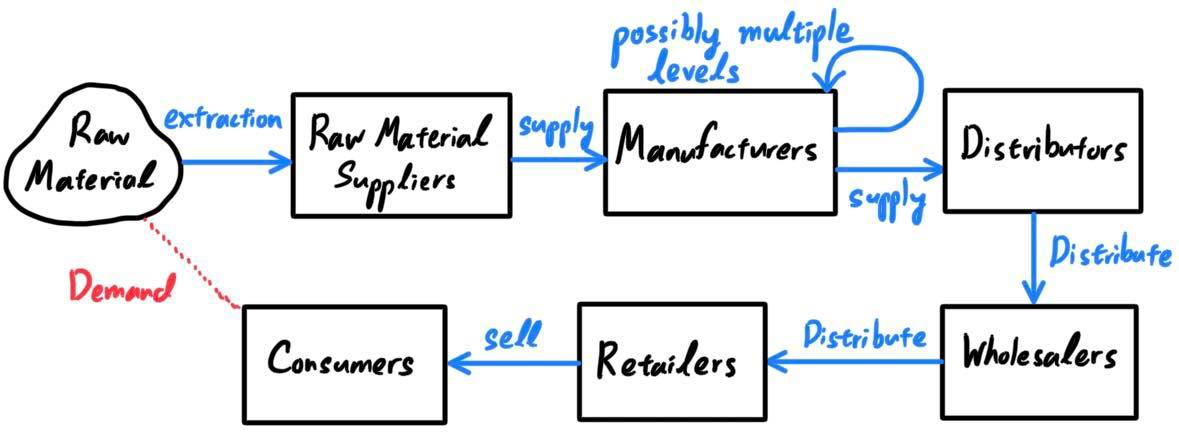
\includegraphics[width=0.9\textwidth]{Images/simplified_supply_chain.jpg}
    \end{center}
    This is just a generic diagram for general supply chains, which may not contain some components or contain extra ones. But note that a fundamental property of supply chains is that with each link, company A must sell to B at a profit, who must sell to C at a profit, and so on, driving up the final price of the good when it gets to retailers. Therefore, skipping the "middleman" gives extra room for more profit for companies and for consumers.

    When thinking of any business (whether it's a retailer, supplier, manufacturer, distributor, etc.), we can interpret it as a function that inputs some set of "things" and outputs "products" that have a higher value in which the company can sell for at a profit. However, the diversity in inputs and outputs make it quite hard to construct a universal model of a business. Generally, if you're running a business within a supply chain, and you must create some product, it's good to think about three types of inputs:

    \begin{enumerate}
      \item \textbf{Inventory} are short-term assets that are direct inputs in the supply chain to produce whatever output. They are not reused. e.g. raw materials for manufacturing, finished products in storage waiting to be sold, land for home building to be sold.
      \item \textbf{Property, Plant, Equipment (PPE)} are long-term assets that are reused and depreciated over time. They aid in the efficient process of producing whatever output. e.g. machinery for manufacturing, trucks for delivery, warehouses for storage, office buildings, land (for office space).
      \item \textbf{Labor} which consists of any and all forms of work done by individuals, can come in many forms. A business can use internal labor (e.g. company employees \& management, internal staff) or external labor (e.g. outsourcing, offshoring, consultants, lawyers, contractors, auditors). A company can hire a full-time lawyer as an internal employee, but many roles are being outsourced these days for increased specialization. The labor force has many jobs, e.g. manual labor, equipment operation, delivery, marketing, HR, management, etc.
    \end{enumerate}

    A visual is shown below. It is important to understand that the arrows pointing into this company \textit{represents some abstract use of the inputs in operational processes}. In most cases, inventory is more of a one-time use while PPE is reused over and over. Labor can be either: one-time use for a certain project through contractors or a consistent job that internal staff performs on the day-to-day basis.

    \begin{center}
    %  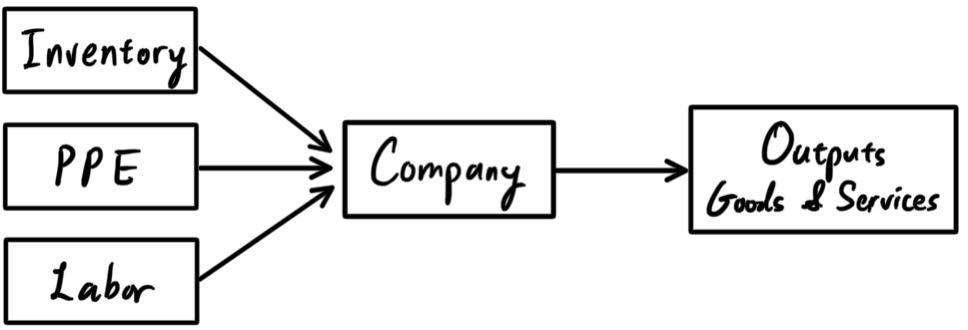
\includegraphics[width=0.95\textwidth]{Images/inputs_of_company.jpg}
    \end{center}

    A final point to make is that the supply chain is more like a network rather than a chain, represented by the visual below. In fact, many companies have \textbf{supply chain managers (SCM)} to oversee that the supplies are streamlined and efficiently moved down.

    \begin{center}
    %  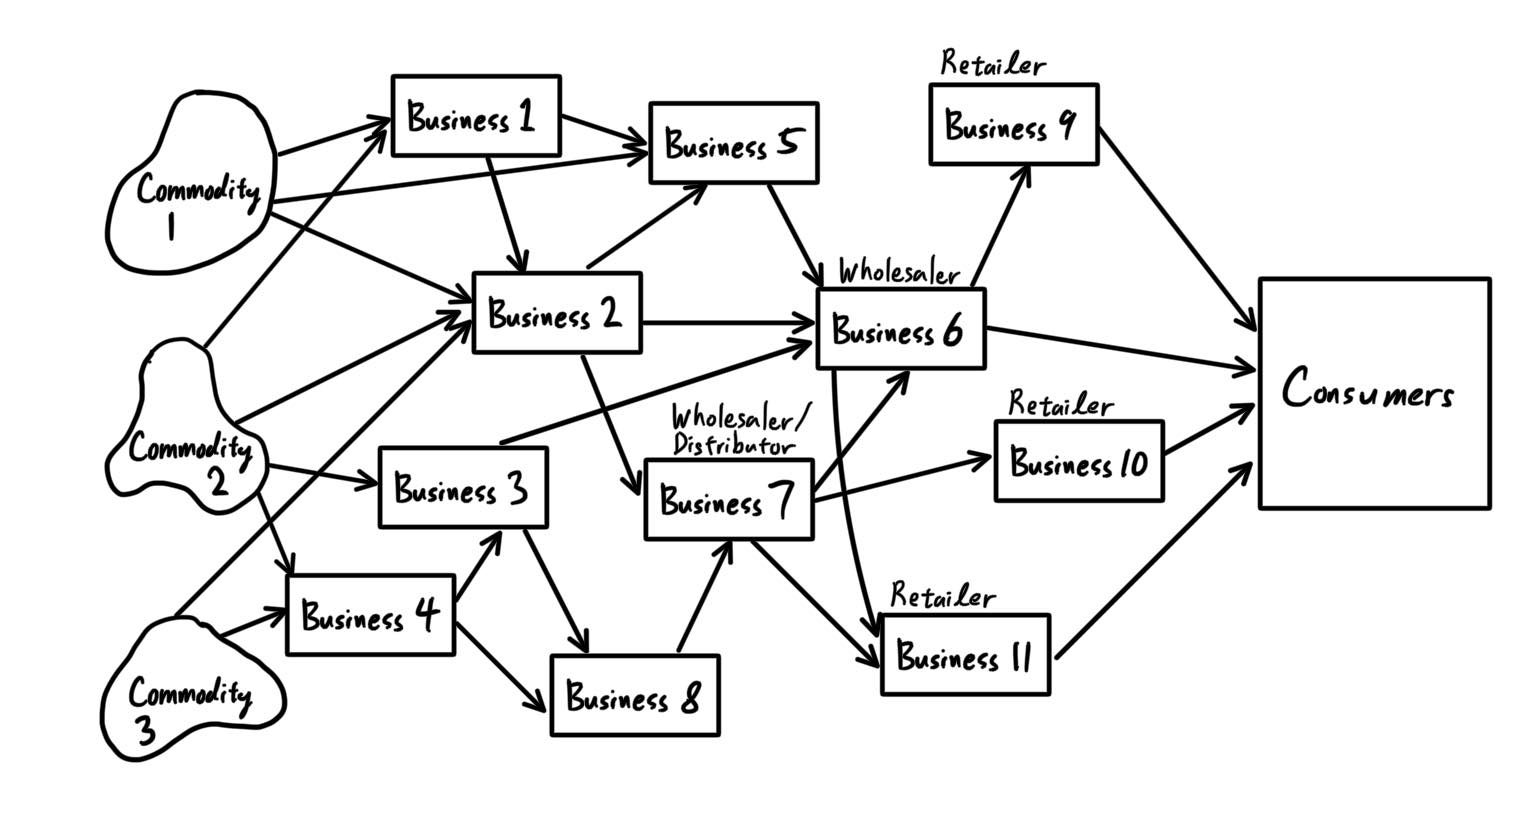
\includegraphics[width=0.95\textwidth]{Images/Supply_Chain_as_Network.jpg}
    \end{center}

  \subsection{Unemployment}

    \begin{definition}[U.S. Department of Labor]
      The \textbf{U.S. Department of Labor (DOL)} is a agency responsible for enforcing federal labor standards and promoting workers' well-being. Some of its purposes are: 
      \begin{enumerate}
          \item It creates employment opportunities, protects retirement and healthcare benefits, help employers find workers, etc. 
          \item It enforces many laws, including the \textit{Fair Labor Standard Act}, which establishes minimum wage standards and overtime pay. 
          \item Oversees the \textbf{Bureau of Labor Statistics (BLS)}, which provides important data such as the unemployment rate, CPI, and PPI. 
      \end{enumerate}
      Every month the BLS conducts the \textbf{Current Population Survey} using a sample of 60,000 households, or around 110,000 individuals. Unemployment rates and other measures are calculated after collection. 
    \end{definition}

    \begin{definition}[Unemployment]
      \textbf{Unemployment} is persons above a specified age (usually 15) not being in paid employment or self-employment but currently available for work during the reference period. The \textbf{Bureau of Labor Statistics} defines it as: 
      \begin{enumerate}
        \item People with jobs are \textit{employed}. 
        \item People who are jobless, looking for a job, and available for work are \textit{unemployed}. 
        \item The \textbf{labor force} is made up of the employed and the unemployed. 
        \item People who are neither employed nor unemployed are \textit{not in the labor force}. 
      \end{enumerate}
      Note that those on active duty in the Armed Forces are not considered in the labor force. Students can be classified as employed, unemployed, or neither, whether they are in school on a full or part-time basis. 
    \end{definition}

    \begin{definition}
      The \textbf{unemployment rate} is the percentage of the labor force that is jobless. It is a \textbf{lagging indicator}, meaning that it generally rises or falls \textit{after} changing economic conditions, rather than anticipating them. 

      There are six ways that the unemployment rate could be calculated: U-1 through U-6: 
      \begin{enumerate}
        \item \textbf{U-1} refers to people who have been unemployed for 15 weeks or longer, expressed as a percentage of the labor force: 
        \[\text{U-1} = \frac{\text{Unemployed 15+ Weeks}}{\text{Labor Force}}\]
        \item \textbf{U-2} refers to people who lost their jobs, or whose temporary jobs ended
        \[\text{U-2} = \frac{\text{Job Losers}}{\text{Labor Force}}\]
        \item The \textbf{U-3 rate} is the most widely used and cited: 
        \[\text{U-3} = \frac{\text{Unemployed}}{\text{Labor Force}}\]
        \item \textbf{U-4} refers to unemployed people, plus discouraged workers
        \[\text{U-4} = \frac{\text{Unemployed + Discouraged}}{\text{Labor Force + Discouraged}}\]
        where \textbf{discouraged workers} are those who are available to work and would like a job, but have given up actively looking for one. 
        \item \textbf{U-5} refers to unemployed people, plus those who are marginally attached to the labor force
        \[\text{U-5} = \frac{\text{Unemployed + Marginally Attached}}{\text{Labor Force + Marginally Attached}}\]
        where \textbf{marginally attached} workers include discouraged workers and anyone else who would like a job and has looked for one in the past 12 months but have given up actively searching. 
        \item \textbf{U-6} refers to unemployed people, plus people who are marginally attached to the labor force, plus those who are employed part-time for economic reasons. 
        \[\text{U-6} = \frac{\text{Unemployed + MA + PTER}}{\text{Labor Force + MA}}\]
        This metric, also called the \textit{real unemployment rate}, is the BLS's most comprehensive. In addition to the categories included in U-5, it accounts for people who have been forced to settle for part-time even though they want to work full-time. This category is called the \textbf{underemployed}. 
      \end{enumerate}
      From this, we can see that by definition
      \[\text{U-1} < \text{U-2} < \text{U-3} < \text{U-4} < \text{U-5} < \text{U-6}\]
    \end{definition}

\section{International Trade}

  \begin{definition}[Imports, Exports]
    A product that is sold to the global market is called an \textbf{export}. A product that is bought from the global market is an \textbf{import}. 
  \end{definition}

  \begin{definition}[International Trade]
    \textbf{International trade}, which is the exchange of goods/services between countries, allows countries to expand their markets and access goods/services that otherwise may not have been available domestically. 

    Global trade allows wealthy countries to use their resources (e.g. labor, technology, or capital) more efficiently. Different countries are endowed with different assets and natural resources, such as land, labor, capital, resources, and technologies. This allows some countries to have a \textit{comparative advantage} over others, and by taking advantage of trade, everyone can benefit. 

    In addition to increased efficiency, international trade allows countries to participate in a global economy, encouraging the opportunity for foreign direct investment. This allows economies to grow more efficiently and to become competitive economic participants. 
  \end{definition}

  International trade has two contrasting views regarding the level of control placed on trade between countries. 

  \begin{definition}[Free Trade]
    The \textbf{free trade} approach, also referred to as \textbf{laissez-faire} economics, place absolutely no restrictions on trade. It states that supply and demand factors, operating on a global scale, will ensure that production happens efficiently. Therefore, nothing needs to be done to protect or promote trade and growth because market forces will do so automatically.

    Elaborating, laissez-faire says that economic competition constitutes a "natural order," also known as the \textit{invisible hand} (by Adam Smith), that rules the world. Furthermore, it is argued that this hand is the best type of regulation, meaning that there is no need for businesses and industrial affairs to be complicated by government intervention. They oppose any federal involvement in the economy, including minimum wages (price floors), duties, trade restrictions, and corporate taxes), viewing them as a penalty for production. 
  \end{definition}

  \begin{definition}[Protectionism]
    \textbf{Protectionism} holds that regulation of international trade is important to ensure that markets function properly. Advocates of this theory believe that market inefficiencies may hamper the benefits of international trade, and they aim to guide the market accordingly. Protectionists support these federal involvements. 
  \end{definition}

  We define some common forms of protectionism. 

  \begin{definition}[Subsidies]
    A \textbf{subsidy} is a direct or indirect payment to individuals or firms, usually in the form of a cash payment from the government or a targeted tax cut. Subsidies are generally seen as a privileged type of financial aid, as they lessen an associated burden that was previously levied against the receiver, or promote a particular action by providing financial support. It is often considered to be in the overall interest of the public, given to promote a social good or an economic policy. Some common types of subsidies are: 
    \begin{enumerate}
      \item \textbf{Welfare payments}, which are government-sponsored assistance programs for individuals and families in need (e.g. health care assistance, food stamps). They are typically funded through taxation. In the U.S., the federal government provides grants to each state through the \textbf{Temporary Assistance for Needy Families (TANF)} program. Eligibility for benefits is based on a number of factors, such as income level and family size. Welfare beneficiaries usually receive a biweekly or monthly payment in the form of food stamps, vouchers, or even direct payments. 
      \item \textbf{Unemployment benefits (aka compensation, income)}, which are temporary government payments to unemployed workers who have lost their jobs due to layoffs or other reasons not of their own fault (business closed, etc.). It is to provide a social safety net to individuals who are looking for a new job. They are often calculated as a percentage of the average of the claimant's pay over a recent 52-week period (subject to income tax). Under normal circumstances, most states pay a maximum of 26 weeks of unemployment benefits, but benefits can be extended or augmented during times of economic crisis. 
      \item \textbf{Subsidized student loans}, which are student loans that have a \textit{subsidized interest rate}. This means that the individual pays for the principal amount, but the government pays the accrued interests. This encourages people to further their education. 
    \end{enumerate}
    Historically, the vast majority of corporate subsidies in the U.S. have gone towards four industries: agriculture, financial institutions, oil companies, and utilities companies. 
  \end{definition}

  \begin{definition}[Stimulus Package]
    A \textbf{stimulus package} is a coordinated effort to increase government spending, and lower taxes and interest rates, to stimulate an economy and lift it out of depression. 
  \end{definition}

  \begin{example}[Unemployment Benefits]
    We list some cases of unemployment benefits:
    \begin{enumerate}
      \item As of 2018, Minnesota had one of the highest maximum weekly benefits amounts at \$683 (up to 26 weeks), with Massachusetts at \$742 (up to 30 weeks). Florida had \$275 maximum weekly benefit for 12 weeks. 
      \item During the Great Recession, unemployment income payments may last for over 100 weeks. During times of low unemployment, such benefits tend to last for up to 26 weeks in most states. 
      \item On March 27, 2020, President Trump signed into law a \$2 trillion coronavirus emergency stimulus package called the \textit{Coronavirus Aid, Relief, and Economic Security (CARES) Act}, which put provisions in place to provide unemployment benefits to unemployed individuals affected by the pandemic. The law also expanded eligibility to allow those who otherwise don't qualify for benefits, including self-employed people, freelancers, and independent contractors. 
    \end{enumerate}
  \end{example}

  \begin{definition}[Tax Deductions, Credits]
    Other types of subsidies include \textbf{tax deductions} and \textbf{tax credits}. \begin{enumerate}
      \item Tax deductions reduce the amount of taxable income
      \item Tax credits reduce the actual amount of tax owed
    \end{enumerate}
  \end{definition}

  \begin{example}[Affordable Care Act]
    The Affordable Care Act, also known as \textit{Obamacare}, is a healthcare reform signed into law by President Obama in March 2010. With the enactment of the ACA, a number of U.S. families became eligible for health-care subsidies, based on household income and size.  The law includes tax credits that lower monthly health insurance bills, and cost-sharing reductions, which reduce out-of-pocket costs. 
  \end{example}

  \begin{definition}[Economic Sanctions]
    A \textbf{sanction} is a penalty levied on another country, or on individual citizens of another country. It is an instrument of foreign policy and economic pressure with the goal being to force a country to alter its behavior without using military threat (which can be expensive and risky). Some common forms of economic sanctions are: 
    \begin{enumerate}
        \item \textbf{Tariffs}, which are taxes imposed on goods imported from country $B$ into country $A$. Upon imposing this tariff, the domestic consumer in $A$ may shy away from the product due to an increase in price, restricting these imports. Two types: 
        \begin{enumerate}
            \item A \textbf{specific/fixed tariff} is levied as a fixed fee based on the type of item, e.g. \$1000 on a car. 
            \item An \textbf{ad-valorem tariff} is levied based on the item value, such as 10\% of the value of the car. 
        \end{enumerate}
        Tariffs may be imposed to raise revenue or to protect domestic industries from foreign competition. This can lead to hurting domestic consumers (due to higher prices), generating tensions, decreased innovation, and possibly even a \textbf{trade war}. 
        \item \textbf{Quotas}, which are limits on how many goods can be either imported from another country or exported to that country. 
        \item \textbf{Embargoes}, which are trade restrictions that prevents a country from trading with another. 
        \item \textbf{Non-Tariff Barriers (NTBs)}, which are non-tariff restrictions on imported goods. Rather than taxing them, governments can require licensing and packaging requirements, product standards, and other requirements. 
        \item \textbf{Asset Freezes (or Seizures)}, which prevents assets owned by a country or individual from being sold or moved. 
    \end{enumerate}
    \textbf{Unilateral} sanctions are acted by a single country, while a \textbf{multilateral one} means that a group of block of countries is supporting its use. Multilateral sanctions are considered less risky, but unilateral sanctions can be very effective if enacted by an economically powerful country. 
  \end{definition}

  \begin{example}[Bill H.R. 850, World vs Iran]
    Blocking a country's exports through an import sanction increases the possibility that the target country will experience a substantial economic burden. On July 31, 2013, the U.S. passed a sanction that blocked Iran from selling any oil abroad because of its nuclear program. This bill followed a year in which Iran's oil exports had already been cut in half by international sanctions. 
  \end{example}

  \begin{example}[U.S. Embargo on Cuba]
    In 1962, the U.S. embargo on Cuba prevented almost all U.S. exports to Cuba. Since the year 2000, the embargo no longer prohibits the trade of food and humanitarian supplies. 
  \end{example}

  \begin{definition}[WTO]
    Sometimes, a government can use a sanction as a way to demonstrate resole or to create a distraction from domestic trouble. To mediate these potentially irresponsible behavior, international organization such as the \textbf{World Trade Organization (WTO)} have panels that objectively review disputes between countries. 

    Moreover, decisions on economic sanctions made by the U.S. are often based on mandates by the United Nations. Allied countries frequently band together, making joint agreements to restrict trade with specific nations. 
  \end{definition}

  Sometimes, sanctions can have drastic unforeseen impacts. 

  \begin{example}[OAPEC Embargo on U.S.]
    The \textit{Organization of Arab Petroleum-Exporting Countries (OAPEC)} issued an embargo on oil shipments to the United States in 1973 as a punishment for resupplying Israel with arms. This caused fuel shortages, rationing, and soaring gas prices. OAPEC was using the embargo as a tool of foreign policy, but the effects later spilled over and exacerbated the worldwide stock market crash of 1973-74. 
  \end{example}

  \begin{example}[Embargoes after 9/11 Attacks]
    In the wake of the September 11 terrorist attacks in 2001, U.S. embargoes were increasingly directed against countries with known ties to terrorist organizations. Lately, U.S. embargoes have become more widespread. 
  \end{example}

  \begin{example}[Trump vs China]
    When President Trump began his term in 2016, he pledged to make it easier to consumers to buy American products. He proceeded to slap import taxes on certain goods entering the country, leading some nations, such as China, to hit back with punitive measures of their own. 
  \end{example}

  \subsection{Imports/Exports \& International Supply Chains}

    A company within a domestic supply chain would find that it may have a limited number of options on where they can get the inputs (labor, PPE, or inventory) or can send the outputs. In fact, it may be cheaper for the company to look at \textbf{international markets} since

    \begin{enumerate}
      \item the inputs may be cheaper to acquire, more so than the additional costs of oversight and transportation
      \item the outputs can be sold for higher profit, more so than the additional costs of oversight and transportation
    \end{enumerate}

    It is a basic economic fact that specialization of labor leads to more efficient production of goods and services. This is due to the \textbf{comparative advantage} of certain countries over others due to geography, climate, technology, and other qualities. Therefore, we are looking at a bigger network of companies participating in an \textbf{international supply chain}. We provide two (out of the many) examples. Say that country A and country B has their supply chains, with A1/B1 wood suppliers, A2/B2 manufacturers, A3/B3 wholesalers, and A4/B4 retailers.

    \begin{enumerate}
      \item A2's POV: If the wood prices in country B are significantly lower (due to, say more forests in country B's geography), then A2 can choose to get its wood from B1 over A1, leading to higher profits when selling it to A3. Furthermore, if the demand for whatever A2 is making is much higher in country B, then A2 can choose to sell it to B3 (or possibly even B4) at a premium, also leading to higher profits.
      \item A3's POV: If there is plenty of cheap labor in country B, company A3 can import inputs from B2 at a cheaper price to sell to A4. If the demand for the product is higher in country B, then A3 can export it back out to sell them at a higher revenue over the transportation costs.
    \end{enumerate}

    \begin{center}
    %  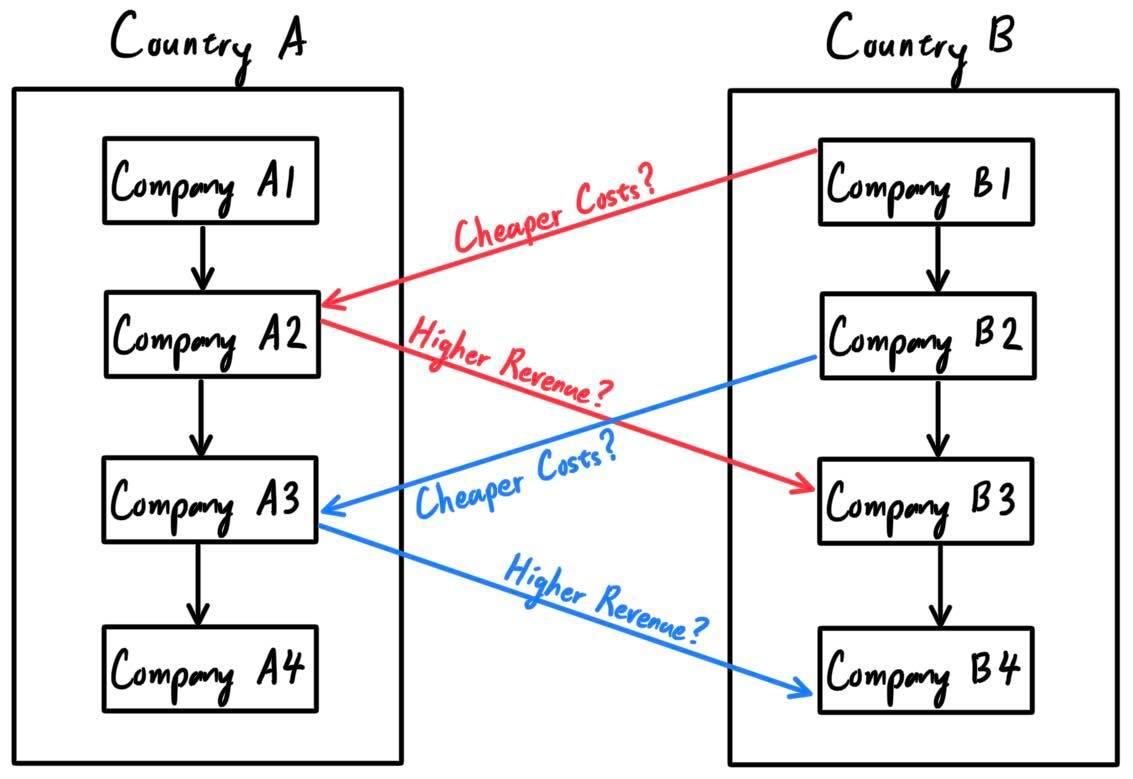
\includegraphics[width=0.9\textwidth]{Images/International_Trade_Examples.jpg}
    \end{center}

    \textbf{International trade} is the exchange of capital, goods, and services across international borders or territories. It is usually more complicated and less mobile than domestic trade.

    For example, England and Portugal have historically both benefited by specializing and trading according to their \textbf{comparative advantages}. Portugal has plentiful vineyards and can make wine at a low cost, while England is able to more cheaply manufacture cloth given its pastures are full of sheep. Each country would eventually recognize these facts and stop attempting to make the product that was more costly to generate domestically in favor of engaging in trade. Indeed, over time, England stopped producing wine, and Portugal stopped manufacturing cloth. Both countries saw that it was to their advantage to stop their efforts at producing these items at home and, instead, to trade with each other in order to acquire them.

    There are two types of trade:
    \begin{enumerate}
      \item An \textbf{export} is a product that is sold to the global market. It is divided into \textbf{product/goods/merchandise exports} and \textbf{service exports}. Any goods \& services (products, materials, labor) that a company sends overseas to another nation in the supply chain is an export.
      \item An \textbf{import} is a product that is bought from the global market. It is divided into \textbf{product/good/merchandise exports} and \textbf{service exports}. Any goods \& services that companies abroad send into the nation in the supply chain is an import.
    \end{enumerate}

  \subsection{International Trade Policies}

    As international trade opens up the opportunity for specialization, and thus more efficient use of resources, it has the potential to maximize a country's capacity to produce and acquire goods. Furthering this point, the \textbf{free trade} theory states that there should be no restrictions on trade, and that supply and demand factors, operating on a global sale, will ensure that production happens efficiently. \textbf{Protectionism} says that regualation of international trade is important to ensure that markets function properly. Countries can impose policies to control trade. Let us use the same model of two countries $A$ and $B$, with their respective companies $A_1, A_2, \ldots$ and $B_1, B_2, \ldots$.
    Say that country $A$ imposes an \textbf{(import) tariff}, in some contexts called an \textbf{(import) duty}, on a certain good from country $B$, which may be a fixed sum or a percentage. If company $A_j$ wants goods from any company $B_i$, then $A_j$ must pay a tax to the federal government of $A$. Note the effects:
    \begin{enumerate}
      \item This can increase government revenue.
      \item This would discourage and limit the imports of this good (since the company $A_j$ wouldn't want to pay more for the same amount of goods), which can improve the economics of producing that product domestically.
      \item This would raise prices for consumers, since the additional cost of importing leads to a subsequent increase in prices all the way through the supply chain.
      \item This can be used as political leverage against countries.
      \item This can lead to lower quality products due to reduced competition.
      \item Foreign companies importing to company $A$ may have an incentive to build factories and offices in country $A$.
    \end{enumerate}

    An \textbf{export tariff/duty} works in the same way: the company exporting a certain good will have to pay a tax to the federal government of the exporting country. This would result in the company exporting them for higher prices in order to make up for the money lost in taxes.
    In the visual, say that company $B_i$ wants to sell USD 1B worth of wood to $A_j$. Normally, the transaction would happen as shown in the top, with USD 1B profit for $B_i$ in exchange for some amount of wood. If country $A$ has a 10\% tariff on wood imports, then after paying the USD 1B, company $A_j$ must pay an \textit{additional} USD 100M to the government $A$. Therefore, if $A_j$ is still buying from $B_i$, it must pay USD 1.1B for the same amount of wood.
    \begin{center}
      %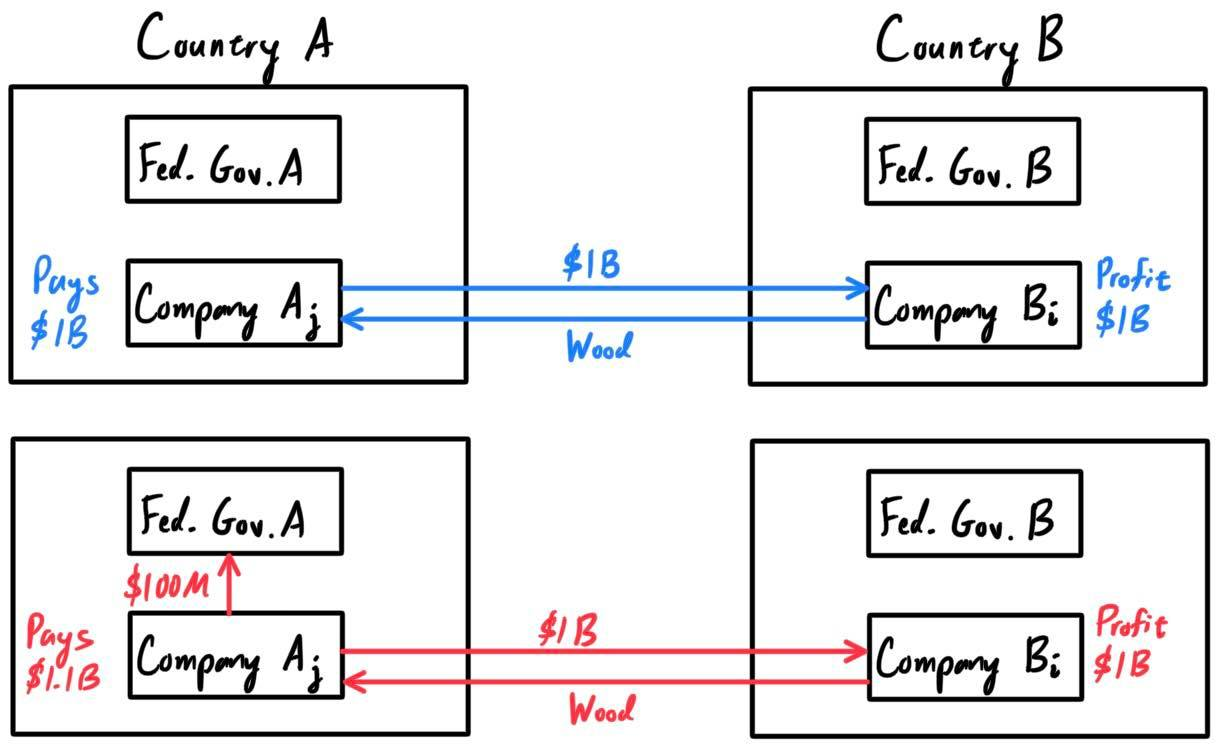
\includegraphics[width=0.9\textwidth]{Images/Import_Tariff.jpg}
    \end{center}

    Say that a certain industry in country A is struggling due to international competition. This may be through lowered prices or cheaper labor, which makes the domestic business not profitable without the subsidy. For example, in the A1/A2/A3/A4 example above, if the B1 wood supplier has such cheap rates that every single manufacturer in country A is getting their goods from imports rather than A1, A1 will be struggling due to foreign competition. The government of country A can give company A1 a \textbf{subsidy}, which is some type of financial assistance.

    It comes in many forms, such as a direct payment of funds to a business or industry, reduced tax rates, and price reductions for required goods/services that can be government supported. This allows needed items to be purchased below the current market rate, resulting in savings for the struggling companies. Note the effects:

    \begin{enumerate}
      \item Industries can receive protection from external competition to protect domestic benefit.
      \item Reduced competition can lead to lower quality products.
    \end{enumerate}
    If there is too much volume of trade, a government can impose a \textbf{quota}, a trade restriction that limits the number or monetary value of goods that a country can import or export during a particular period. The purposes of quotas are very similar to that of tariffs (to protect domestic production and political leverage) and can have the same drawbacks (higher prices for consumers, lower quality products due to decreased competition). Generally, quotas are more effective in restricting trade than tariffs but may be more disruptive to international trade.

  \subsection{Currency \& Foreign Exchange}

    As we have mentioned in its history, \textbf{currency} is a medium of exchange for goods and services, issued by a government and generally accepted at its face value as a method of payment (even though fiat money has no intrinsic value).

    The federal government of many nations issue their own currency. This allows each nation to control their own monetary policy through increasing or restricting the supply of money within its national economy. If the entire world had one currency, the entity controlling the production and flow of that currency would have monetary power over the entire world. Having multiple federal banks would also not work, since there may be conflicts of interest.

    About 180 national currencies are recognized by the United Nations, while another 66 countries either use the U.S. dollar or peg their currencies directly to the dollar.

    \begin{enumerate}
      \item the United States has the US Dollar USD
      \item Canada has the Canadian Dollar (CAD)
      \item China has the Chinese Yuan (CNY or RMB)
      \item Japan as the Japanese Yen (JPY)
      \item Korea has the Korean Won (KRW)
      \item Switzerland has the Swiss Franc (CHF)
      \item the UK has the Great Britain Pound Sterling (GBP)
      \item Poland has the Polish Zloty (PLN)
      \item The EU nations, such as Austria, Belgium, Estonia, Finland, France, Germany, Greece, Ireland, Italy, Latvia, Luxembourg, Netherlands, Portugal, Spain, etc., have the euro (EUR).
    \end{enumerate}

    Given all these countries with their own currencies, the natural step is to develop some way to exchange one currency for another. This \textbf{foreign exchange}, shortened to \textbf{forex}, is a requirement for international trade and travel, since goods and services would travel across borders, and one would want a way to convert the value of a foreign good in foreign currencies to that of domestic currencies. Therefore, given nation A with currency AAA and nation B with currency BBB, we can define the \textbf{exchange rate} AAA/BBB to be the number of BBB currency we would need to exchange it for 1 AAA. This is obvious when considering it as a fraction. Say the exchange rate is $k$. Then,

    \begin{equation}
      AAA/BBB = \frac{AAA}{BBB} = k \implies 1 ; AAA = k ; BBB
    \end{equation}

    Foreign exchange transactions take place on the \textbf{forex market}, which is the largest, most liquid market in the world, with trillions of dollars changing hands every day running 24 hours a day (e.g. ~\$6.6T/day in April 2019). It does not have a centralized locations such as national markets or stock exchanges: rather, it is an electronic network of central/commercial banks, brokers, institutions, and individual traders (mostly trading through brokers or banks).
    But how are these exchange rates determined in the first place, and what factors cause them to fluctuate? Let there exist nations A and B with respective currencies AAA and BBB.

    \begin{enumerate}
      \item If B has higher rate of inflation than A, then AAA/BBB would rise. We're really comparing the value of AAA to BBB by looking at their purchasing power of a basket of goods determined by the CPI.
      \item Adding on from above, any increase in the money supply of a nation will depreciate its value. It's common sense that as the money supply increases, its purchasing power will decrease due to inflation.
      \item If the federal government of B increases interest rates, then it offers lenders a higher return relative to other countries. Therefore, countries like A would want to convert their currencies into BBB to invest in B. A high demand for BBB's currency can cause the value of BBB to appreciate.
      \item A country that have a large public debt will suffer a depreciation of its currency. A large debt will eventually have to be serviced and paid off with cheaper real dollars in the future, which may happen through printing money (which increases money supply and causes inflation). Foreigners may also be scared off by large debts also due to a risk of national default on loans.
      \item A country that is politically stable and has a strong economic performance will draw foreign investors looking for safe, credit-worthy investments.
    \end{enumerate}

    The results of exchange rates can be described as such: If the exchange rate AAA/BBB rises, then this is generally good for nation A and bad for B. Since AAA's worth (relative to BBB) has gone up, A's imports from B will be cheaper for A and A's exports to B will be more expensive for B. This means that A's companies' income from exports will increase and expenditure from imports will decrease.

    \begin{enumerate}
      \item For example, let B be a major exporter of oil to A, with the exchange rate $AAA/BBB = 1$. If a barrel of oil is 60 BBB, then (ignoring transportation \& operational costs) a company in A could buy oil for 60 AAA, which would convert to the correct price of 60 BBB. Now, assume that the exchange rate is changed to $AAA/BBB = 1.2$. This means that a company in A can pay 50 AAA, which is worth 60 BBB, for a barrel of oil. This makes the import purchase cheaper for A.
      
      \begin{center}
        % 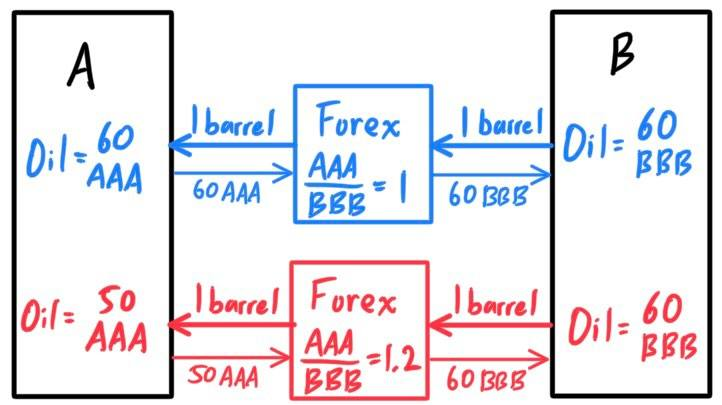
\includegraphics[width=0.9\textwidth]{Images/forex_barrel.jpg}
      \end{center}

      \item Furthermore, if A is an exporter of, say timber, to B, with timber prices at 100 AAA per ton, then a company in B could originally buy the ton with 100 BBB. With the increased exchange rate, a company in B would have to pay 120 BBB (which translates to 100 AAA) to import a ton of timber from A. Therefore, B would have to increase their payment from 100 BBB to 120 BBB to get the same goods and services from A, which increases their expenditures on imports.

      \begin{center}
        % 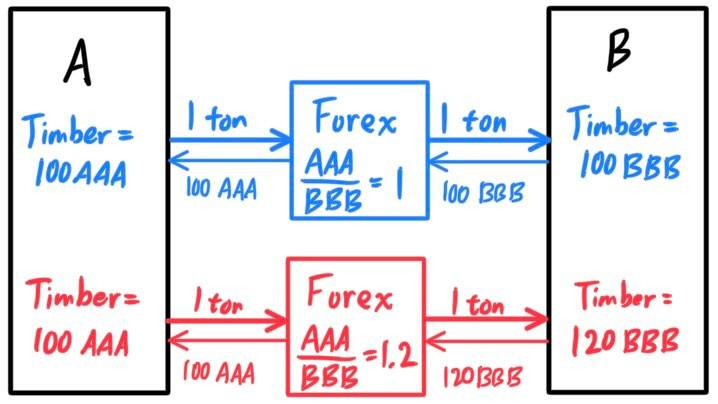
\includegraphics[width=0.9\textwidth]{Images/forex_timber.jpg}
      \end{center}
    \end{enumerate}

    A strong currency is not always the best thing for a country. On the one hand, if a currency apprecaites, all of its imported goods get a lot cheaper. If a country tends to import a lot more goods than they export, then an appreciated currency might be desirable. But on the other hand, if a country relies heavily on exports, an appreciating currency isn't such a great thing. When A's currency appreciates, it is more expensive for other countries to import A's goods/services and so international trade will decrease.

    Many nations have their own currencies that vary in value depending on the overall strength of the economy and policies. However, a nation may \textbf{peg its currency} to that of another nation. A \textbf{currency peg} is a policy in which a national government sets a specific fixed exchange rate of its currency with a foreign currency (usually the USD or euro), done by actively controlling the value of the currency so that it rises and falls along with the dollar. Nation B might peg its currency to that of (usually a more developed) nation A to encourage trade between the two countries by reducing foreign exchange risk. This is especially important when profit margins for many businesses in B are low, so small shifts in exchange rates can eliminate profits and force firms to find new suppliers.

    To maintain the dollar peg, a nation B's central bank must have a large \textbf{foreign reserve}. As a result, most of the countries that use a USD peg have significant exports to the United States. B's companies receive lots of dollar payments, which they exchange for local currency BBB with B's central bank to pay their workers and domestic suppleirs. B's federal government amasses its foreign reserve of US dollars this way. This fund is further grown by buying U.S. Treasuries to receive interest on their dollar holdings.

    \begin{center}
      % 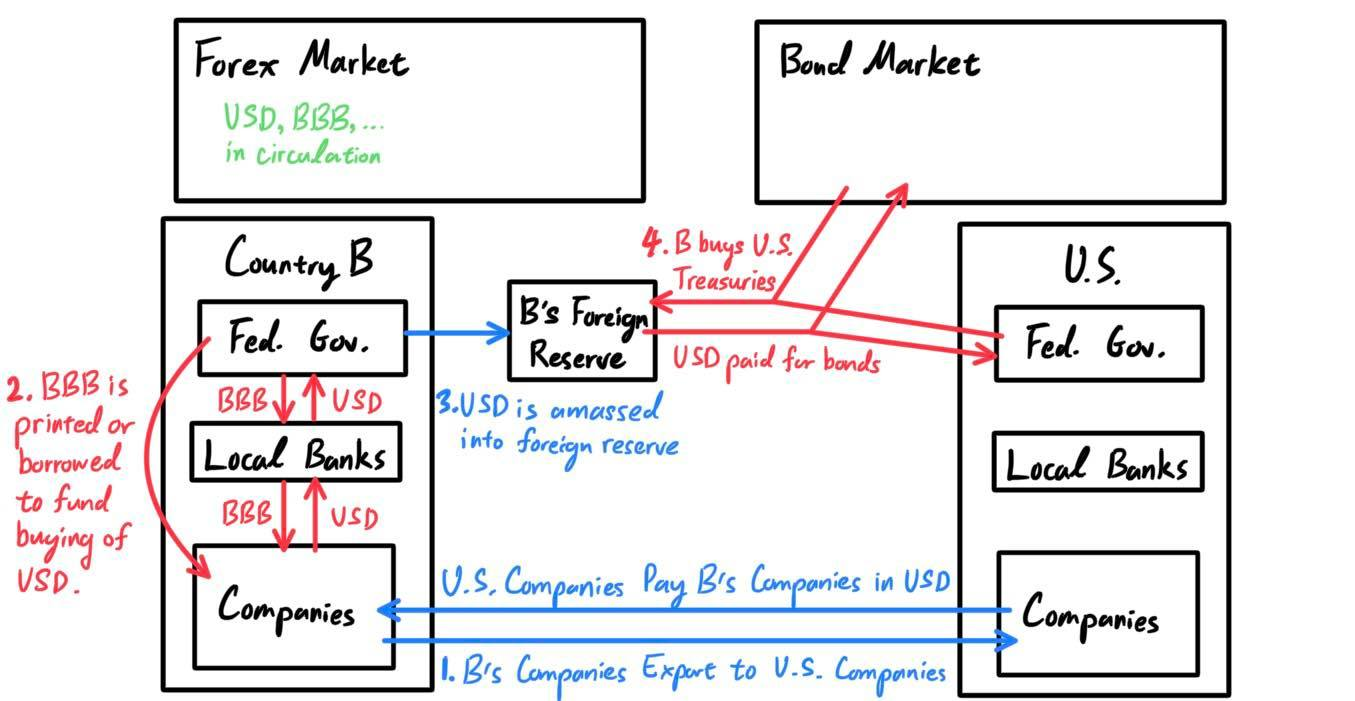
\includegraphics[width=0.95\textwidth]{Images/dollar_peg_1.jpg}
    \end{center}

    If BBB/USD falls below the peg, then B must raise its value and/or lower the dollar's value. It does this by selling Treasuries on the secondary market and receiving USD to purchase its currency from the forex market. The reduced supply of BBB in the forex market raises its value. Furthermore, the selling of treasuries in the bond market adds to its supply, resulting in a drop in value of the bond along with the value of the dollar.

    \begin{center}
      % 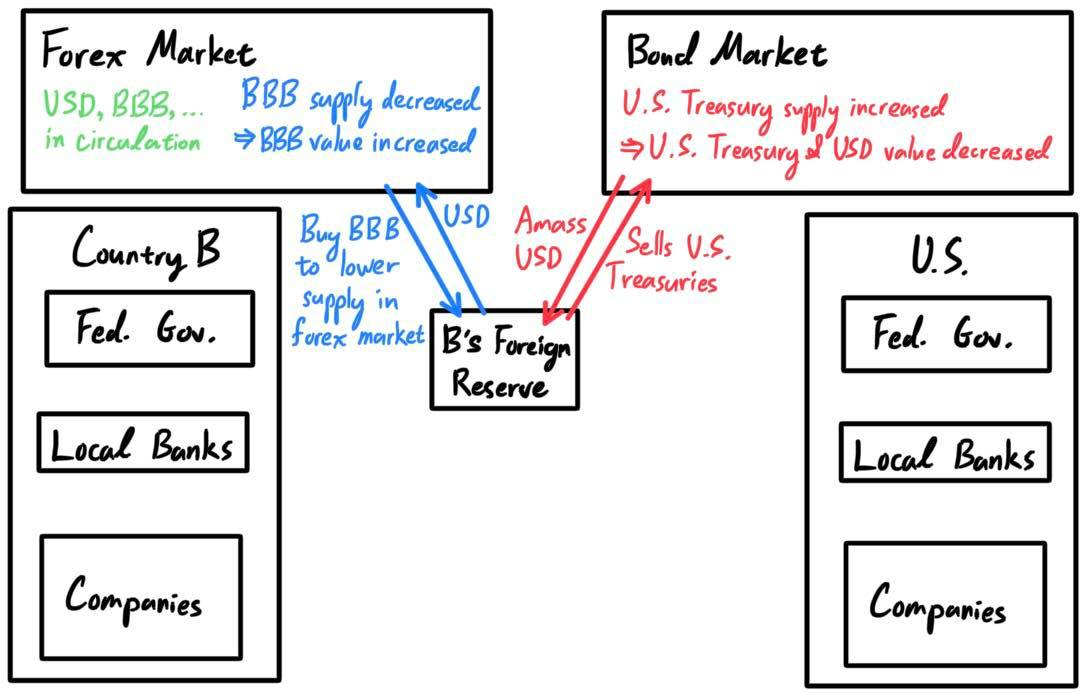
\includegraphics[width=0.95\textwidth]{Images/dollar_peg_2.jpg}
    \end{center}

    \begin{enumerate}
      \item One example is China, which prefers to keep its currency low to make its exports more competitive. It does it like this: China's currency power comes from its exports to America. Chinese companies receive USD as payment for their exports, which they deposit into their banks in excahnge for Yuan to pay their workers. Local Chinese banks transfer dollars to China's central bank, which stockpiles them in its foreign currency reserves. The Chinese central bank holdings reduce the supply of dollars available for trade, putting upward pressure on the dollar. This will further strengthen the dollar and lower the Yuan's value.
    \end{enumerate}

\section{National Income Accounting}

  \begin{definition}[Gross Domestic Product]
    If we think of a nation as a giant firm that takes in inputs and produces outputs, then the \textbf{gross domestic product (GDP)} is the total monetary or market value of all the finished goods and services produced within a country's borders in a specific time period. As a broad measure of overall domestic production, it functions as a comprehensive scorecard of a given country's economic health within the international market. It is typically calculated on an annual basis (\textit{annualized GDP}), and sometimes on a quarterly one. There are multiple ways we can measure GDP: 
    \begin{enumerate}
      \item \textbf{Nominal GDP} does not take into account inflation. It is an assessment of economic production in terms of the current prices of goods and services.  
      \item \textbf{Real GDP} does take inflation into account, allowing it to be measured in current dollars. 
      \item \textbf{GDP Growth} compares the year-over-year change in a country's economic output in order to measure how fast an economy is growing, expressed as a percentage rate. If GDP growth rates accelerate, it may be a signal that the economy is "overheating" and the central bank may seek to raise interest rates. Conversely, a shrinking (or negative) GDP growth rate is a signal that rates should be lowered and that stimulus may be necessary. 
      \item \textbf{GDP Purchasing Power Parity (PPP)} is a method to see how one country's GDP measures up in "international dollars" using a method that adjusts for differences in local prices and costs of living in order to make cross-country comparisons. 
      \item \textbf{GDP per capita} is a measurement of the GDP per person in a country's population. It indicates the amount of output or income per person in an economy and can indicate average productivity or average living standards. GDP per capita can be stated in nominal, real, or PPP terms. 
    \end{enumerate}
  \end{definition}

  There are three ways of calculating the GDP of a nation, all of which should theoretically add to the same value. 
  \begin{enumerate}
    \item Production Approach
    \item Income Approach
    \item Expenditure Approach
  \end{enumerate}

  \begin{definition}[Expenditure Approach]
    The \textbf{expenditure/spending approach} calculates spending by the different groups that participate in the economy. It can be calculated using the following formula: 
    \[GDP = C + G + I + NX\]
    where
    \begin{enumerate}
        \item $C = $ Consumption; This refers to private consumption expenditures or consumer spending. Consumers spend money to acquire goods and services, such as groceries and haircuts (which are goods and services produced). Consumer spending is the biggest component of GDP, accounting for more then $2/3$ of the U.S. GDP. Consumer confidence, therefore, has a very significant bearing on economic growth. 
        \item $G = $ Government Spending; This represents government consumption expenditure and gross investment. For example, governments spend money on equipment, infrastructure, and payroll. 
        \item $I = $ Investment; This refers to private domestic investment or capital expenditures (i.e. company expenditures). Businesses spend money in order to invest in their business activities, such as buying machinery. 
        \item $NX = $ Net exports (which is Exports$-$Imports) All expenditures by companies located in a given country, even if they are foreign companies, are included in this calculation. 
    \end{enumerate}
  \end{definition}

  There is another important economic measurement of a country. 

  \begin{definition}[Gross National Income]
    The difference between GDP and \textbf{Gross National Income (GNI)} is that GDP defines its scope according to location, while GNI defines its scope according to ownership. That is, GNI is product produced by enterprises owned by a country's citizens, even in foreign countries.

    It is clear to see by definition 
    \begin{align*}
        GNI = GDP & + (\text{income receipts from the rest of the world}) \\
        & - (\text{income payments from the rest of the world})
    \end{align*}
  \end{definition}

  Split. 

  The \textbf{gross domestic product (GDP)} is the total monetary or market value of all the finished goods and services produced within a country's borders in a specific time period (usually a year). It is a broad measure of overall domestic production and a country's economic health. There are many way to calculate it.

  The \textbf{expenditure approach} says that everything that the private sector (e.g. consumers and private firms) and the government spend within the borders of a particular country must add up to the total value of all finished goods and services produced over a certain period of time. The formula is

  \begin{equation}
    \text{GDP} = \text{C} + \text{I} + \text{G} + (\text{X} - \text{M})
  \end{equation}
  where
  \begin{enumerate}
    \item $C$ is consumer spending on goods and services. Consumers spending money to acquire goods and services, such as groceries and haircuts. It accounts for the majority of the U.S. GDP, more than 2/3, meaning that it is an essential part of GDP. A high confidence levels indicates that consumers are willing to spend, while a low confidence level reflects uncertainty about the future and an unwillingness to spend.
    \item $I$ is investor spending on business capital goods, i.e. capital expenditures on assets with useful lives of more than one year each, such as real estate, equipment, production facilities, and plants.
    \item $G$ is government spending on public goods and services, such as public equipment, infrastructure, and payroll (basically federal spending).
    \item $X$ is exports and $M$ is imports, and so $X - M$ is the net exports.
  \end{enumerate}

  Note that this model neatly partitions the expenditures of the entire nation, which we can see from observing a few supply chains. Given a completely domestic supply chain of companies, each company would add some value to the product through collecting, manufacturing, packaging, distributing, etc., which is realized through its increasing price as it moves down each link. At the end of the chain, the final value of the product is really the conglomeration of all the incremental values added by each company, representing the total value created by all the companies. Whether this goes to consumers (contributing to $C$) or foreigners (contributing to $X$) depends on where the product is sold. Sometimes, an unfinished product may be exported to be completed in foreign lands. In this case, the value added only up until export would be accounted for in the GDP, contributing to $X$.
  \begin{center}
    %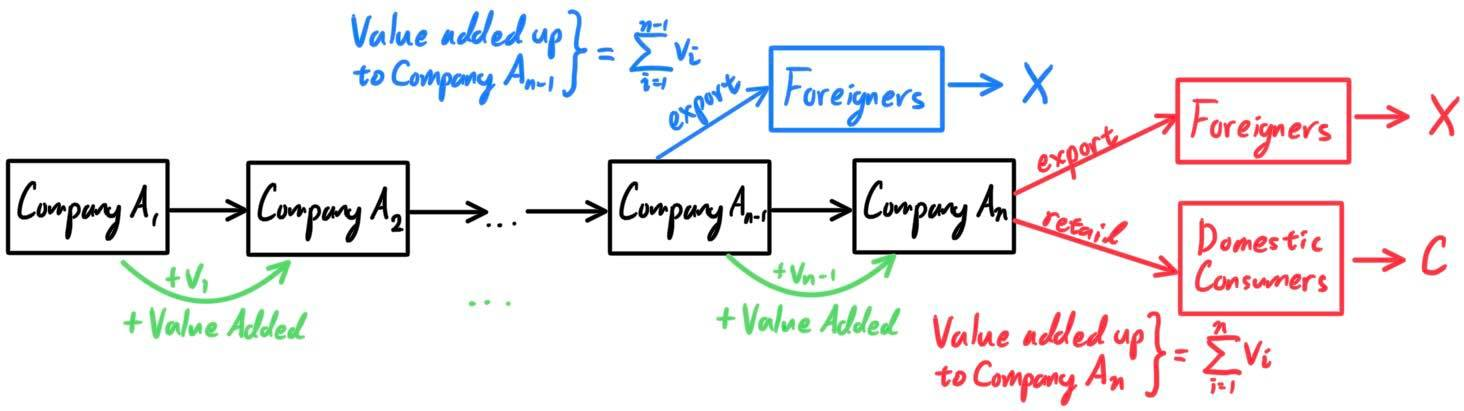
\includegraphics[width=0.95\textwidth]{Images/GDP_1.jpg}
  \end{center}
  Note that at any point, even in the middle of the chain, certain inputs or outputs may go in and out of the chain. If an import is received and travels down to the chain to be sold to the domestic market, the final price of the good includes both the value added by foreign businesses and by domestic ones. This is why the imports \$M\$ are subtracted, which would give us the value only added by domestic businesses.
  \begin{center}
    %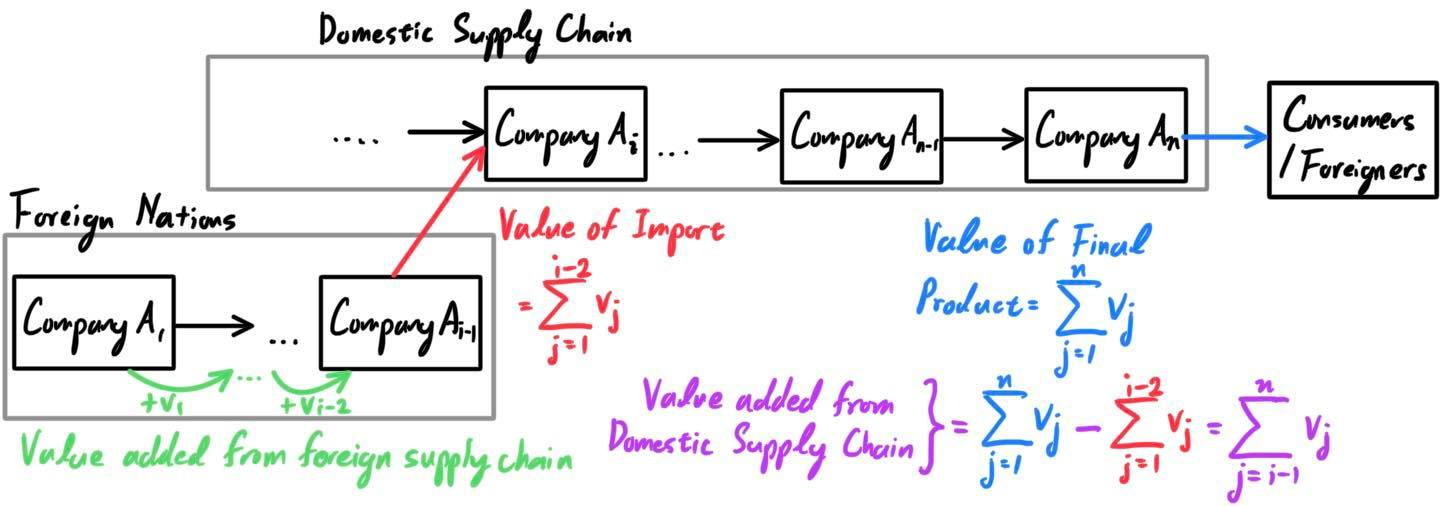
\includegraphics[width=0.95\textwidth]{Images/GDP_2.jpg}
  \end{center}
  Companies can add value through the goods and services they provide, whether it's to domestic consumers or foreign exports. Another addition of value is to the \textit{business itself} (rather than the value of what it creates). When investors invest in businesses directly, the extra capital can be used to buy PPE and other long-term assets, ultimately adding to the value of the nation as a part of \$I\$.
  \begin{center}
    %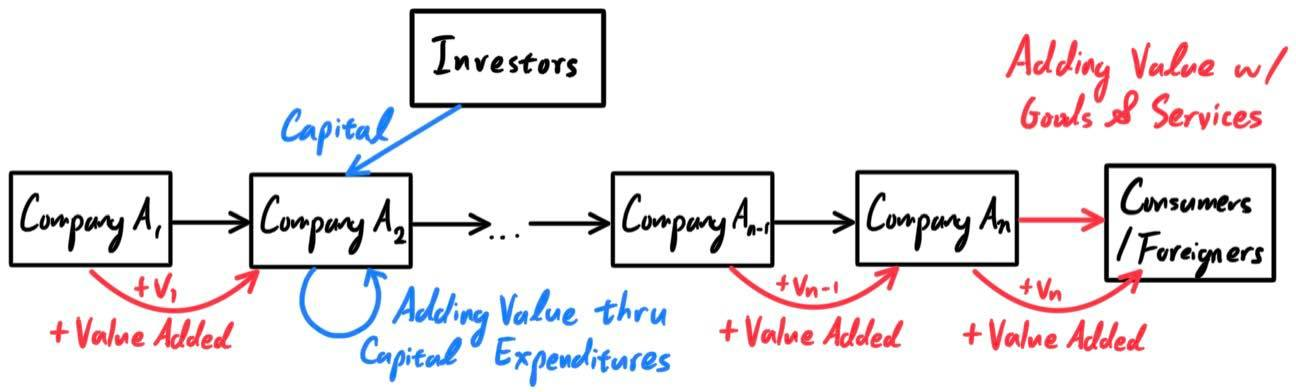
\includegraphics[width=0.95\textwidth]{Images/GDP_3.jpg}
  \end{center}
  It is quite straightforward that government spending contributes to the public by adding value to (mainly) public sectors and projects. The repairing of a highway or building of a new elementary school does indeed add value to the nation, contributing to \$G\$.
  There are actually a couple forms of GDP:

  \begin{enumerate}
    \item \textbf{Nominal GDP} is the raw value of GDP, unadjusted for inflation.
    \item \textbf{Real GDP} is the GDP adjusted for inflation, making it a more accurate indicator for economic growth. It is conventional to use this, which is also called \textbf{GDP in constant USD}.
    \item \textbf{GDP per capita} (nominal or real) is the GDP divided by the population, which produces the average output of an individual within a nation. This is used to normalize the GDP across population when comparing nations.
    \item \textbf{GDP growth rate} compare the year-over-year (or quarterly) change in a country's GDP to measure how fast its economy is growing.
  \end{enumerate}

  We take a look at historical data on the (real) GDP of a few nations:

  \begin{figure}[H]
    \centering 
    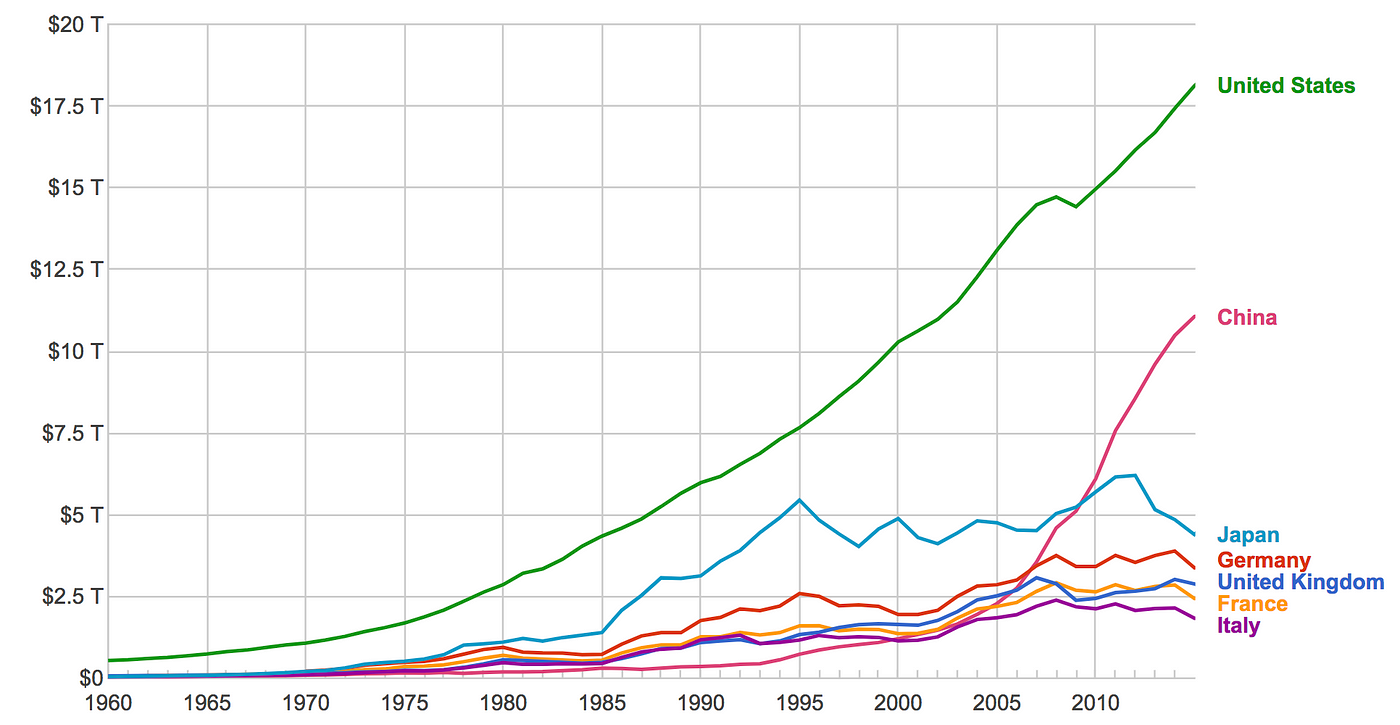
\includegraphics[scale=0.25]{img/GDP.png}
    \caption{GDP of countries. } 
    \label{fig:GDP_data}
  \end{figure}

\section{Inflation}

  \begin{definition}[Inflation]
    \textbf{Inflation} is a measure of the rate of the rising prices of goods and services in an economy. It can occur in nearly any product/services, including need-based expenses such as housing, food, medical care, etc. 

    There are various factors that can drive inflation: 
    \begin{enumerate}
      \item \textbf{Cost-Push Inflation} occurs when prices increases due to increases in production costs, such as raw materials and wages. The demand for goods is unchanged while the supply of goods declines due to the higher costs of production. As a result, the added costs of production are passed onto consumers in the form of higher prices for the finished goods. 
      \item \textbf{Demand-Pull Inflation} can be caused by strong consumer demand for a product or service. When there's a surge in demand for goods across an economy, prices increase, and the result is demand-pull inflation. As the demand for a particular good or service increases, the available supply decreases. When fewer items are available, consumers are willing to pay more to obtain the item—as outlined in the economic principle of supply and demand. The result is higher prices due to demand-pull inflation.
      
      Consumer confidence tends to be high when unemployment is low, and wages are rising—leading to more spending. Economic expansion has a direct impact on the level of consumer spending in an economy, which can lead to a high demand for products and services.
    \end{enumerate}

    Inflation at a moderate amount is healthy for the economy, but it can be a concern because it erodes a consumer's purchasing power and can even interfere with the ability to retire. 
  \end{definition}

  \begin{figure}[H]
    \centering 
    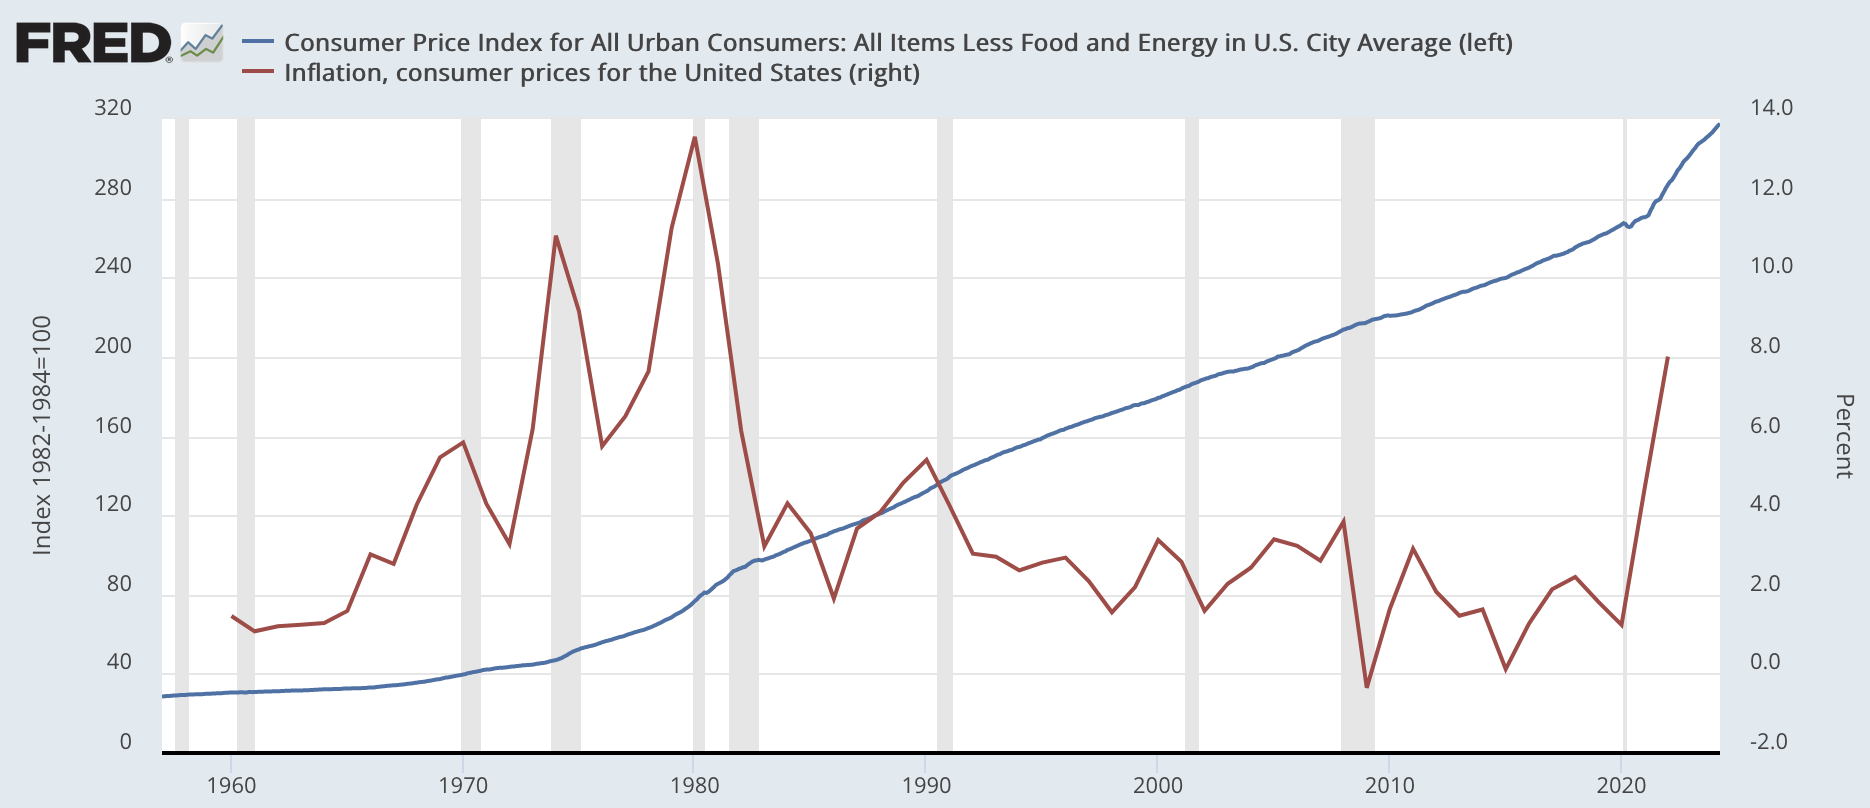
\includegraphics[scale=0.4]{img/inflation_cpi.png}
    \caption{Inflation and consumer price index in the U.S.} 
    \label{fig:inflation_cpi}
  \end{figure}

  \begin{example}[Cost-Push Inflation]
    One of the signs of possible cost-push inflation can be seen in rising commodity prices such as oil and metals since they're major production inputs. For example, if the price of copper rises, companies that use copper to make their products might increase the prices of their goods. The business will pass on the higher costs of raw materials to consumers. The result is higher prices for consumers without any change in demand (but rather a change in supply). 

    Wages also affect the cost of production and are typically the single biggest expense for businesses. When the economy is performing well, and the unemployment rate is low, shortages in labor or workers can occur. Companies, in turn, increase wages to attract qualified candidates, causing production costs to rise for the company. If the company raises prices due to the rise in employee wages, cost-plus inflation occurs. 

    Natural disasters can also drive prices higher. For example, if a hurricane destroys a crop such as corn, prices can rise across the economy since corn is used in many products.
  \end{example}

  \begin{example}[Demand-Pull Inflation from Corporations]
    Companies also play a role in inflation, especially if they manufacture popular products. A company can raise prices simply because consumers are willing to pay the increased amount. Corporations also raise prices freely when the item for sale is something consumers need for everyday existence, such as oil and gas. However, it's the demand from consumers that provides the corporations with the leverage to raise prices.
  \end{example}

  \begin{example}[Housing Market]
    The housing market, for example, has seen its ups and downs over the years. If homes are in demand because the economy is experiencing an expansion, home prices will rise. The demand also impacts ancillary products and services that support the housing industry. Construction products such as lumber and steel, as well as the nails and rivets used in homes, might all see increases in demand resulting from higher demand for homes.
  \end{example}

  There are two main ways to measure inflation. 

  \begin{definition}[Consumer Price Index]
    The \textbf{Consumer Price Index (CPI)} is a measure that examines the weighted average of prices of a basket of consumer goods and services, such as transportation, food, and medical care. It is calculated by taking the average change in prices over time that consumers pay for a basket of goods and services, and it is associated with the cost of living. 
  \end{definition}

  \begin{definition}[Producer Price Index]
    The \textbf{Producer Price Index (PPI)} is a measure that reports the average price changes from domestic production over time. It is different from the CPI in that is measures costs from the viewpoint of industries that make the products, whereas the CPI measures prices from the perspective of consumers. 
  \end{definition}

  \begin{example}[PPI of Balloons]
    The PPI has a base number of 100, which represents no change in prices. If the production of balloons has a PPI of 115 for the month of July, the 115 figure indicates that it cost the balloon manufacturing industry 15\% more to produce balloons in July than it did in June. 
  \end{example}

  Note that companies can both benefit and be hurt by inflation. They can charge more for their products as a result of a surge in demand for their goods, increasing their profit margins, or they can lose money by a surge in production costs (and they cannot pass on the higher costs to consumers through higher prices). 

\section{Monetary Policy}

    The most common principle in finance is that money has a time value. If you were to get \$1 today or \$1 in one year, you should always pick \$1 today since you can take that dollar and deposit it had a bank to receive interest for a year.\footnote{We will assume interest rates to always be nonnegative, though there are some nontrivial cases where it is negative.} To set up the proper terminology without assumption of knowledge, let's walk through a hypothetical scenario. 

    Say that party A wants to borrow $X$ dollars from party B. There are some factors to consider here. First, for what period of time will A borrow from B? This is easily agreed upon between the two. Second, what is the interest rate that B will charge A for borrowing? This is dependent on multiple factors, but it ultimately follows the basic principle that riskier loans require higher interest rates. 
    \begin{enumerate}
      \item If A has good \textbf{creditworthiness}, then B should charge lower interest rates since the risk of default\footnote{This means not being able to pay back a loan.} is low.\footnote{How one's creditworthiness is determined is a whole other subject, so we will assume that this is known and not delve into the how. }
      \item If the length of time $T$ that A borrows money is longer, then the risk of default may be longer, so interest rates should be higher. 
      \item What are interest rates for other types of loans? Depending on the context on say the interest rate similar loans, the parties should agree on some reasonable price.  
    \end{enumerate} 
    There's a couple questions here (beyond how credit is determined). First, how do we quantify how riskier a longer loan is? If you borrow for 2 years vs 1 year, what should the interest rate be? Second, how are other comparable interest rates determined? More generally, how does the third point even work? It looks like we need more background, both qualitative and quantitative to elaborate on all these things. 

  \subsection{Interest Rates} 

    The amount of money loaned $X$ is called the \textbf{principal}, and the interest rate $r$ is represented as a percentage of the principal that needs to be payed in addition \textit{per year}. Therefore, the total amount of money A must pay to B at the end of $t$ years is 
    \begin{equation}
      X (1 + r)^t
    \end{equation} 
    Simple enough, but this model assumes that the loan compounds annually. This may not hold for certain loans, so really if we assume that across the whole $T$ years it is compounded $m$ times, then the total now becomes 
    \begin{equation}
      X (1 + r/m)^{mt}
    \end{equation}

    Using the fact that 
    \begin{equation}
      \lim_{n \rightarrow \infty} \bigg( 1 + \frac{1}{n}\bigg)^n = e
    \end{equation}
    we can model this with a continuous interest rate. 
    \begin{equation}
      X e^{rt}
    \end{equation}
    It is important to comfortably switch between these two types. The market is always effectively discrete since daily compounding is the highest practical frequency in loans, but continuous compounding (exponential growth) is often mathematically more convenient. 

    Now note the goals of the two parties A and B. 
    \begin{enumerate}
      \item A wants to minimize interest rate payment, so if A finds another lender with lower interest rate (with all else equal), then A will go to the new lender. 
      \item B wants to maximize interest rate payment, so if B finds another borrower willing to tolerate a higher interest (with all else equal, like creditworthiness), then B will lend to the new borrower. 
    \end{enumerate}

    There is borrower that everyone has access to: the U.S. government (or could be some other entity). This entity is considered \textbf{risk-free}, meaning that they are guaranteed to give you back your money and so is the ideal place to lend to, with their own interest rate $r_f$ ($f$ for risk-\textbf{f}ree). Therefore, if you are a lender, you should always charge a rate higher than $r_f$, since if it was lower, you can get higher interest (\textit{and} better creditworthiness) by simply lending to the U.S. government. If you are a borrower, you should expect to pay more than $r_f$. Therefore we've essentially lower bounded all interest rates by $r_f$. 
    \begin{equation}
      r > r_f
    \end{equation}
    Again, this only holds true given that everything else is equal, such as the time of borrowing. One person might ask why the government doesn't lower its own interest rates even further? By doing this, the government can save money by having to pay less interest. This is true, but this assumes that the government is trying to make a profit, which is not true. The government controls the flow of money, and setting this risk free rate is strictly to do that. 

    \begin{example}[Home Loans]
      \textbf{Mortgages} are loans to individuals to buy a house, which last either 15 years and 30 years. Historically, the home loan rates are documented below\footnote{The shaded areas represent economic recessions.}, where we can see that the 30 year rates are consistently higher. In order to understand why rates are the way they are, we will need to read further. 
      \begin{figure}[H]
        \centering 
        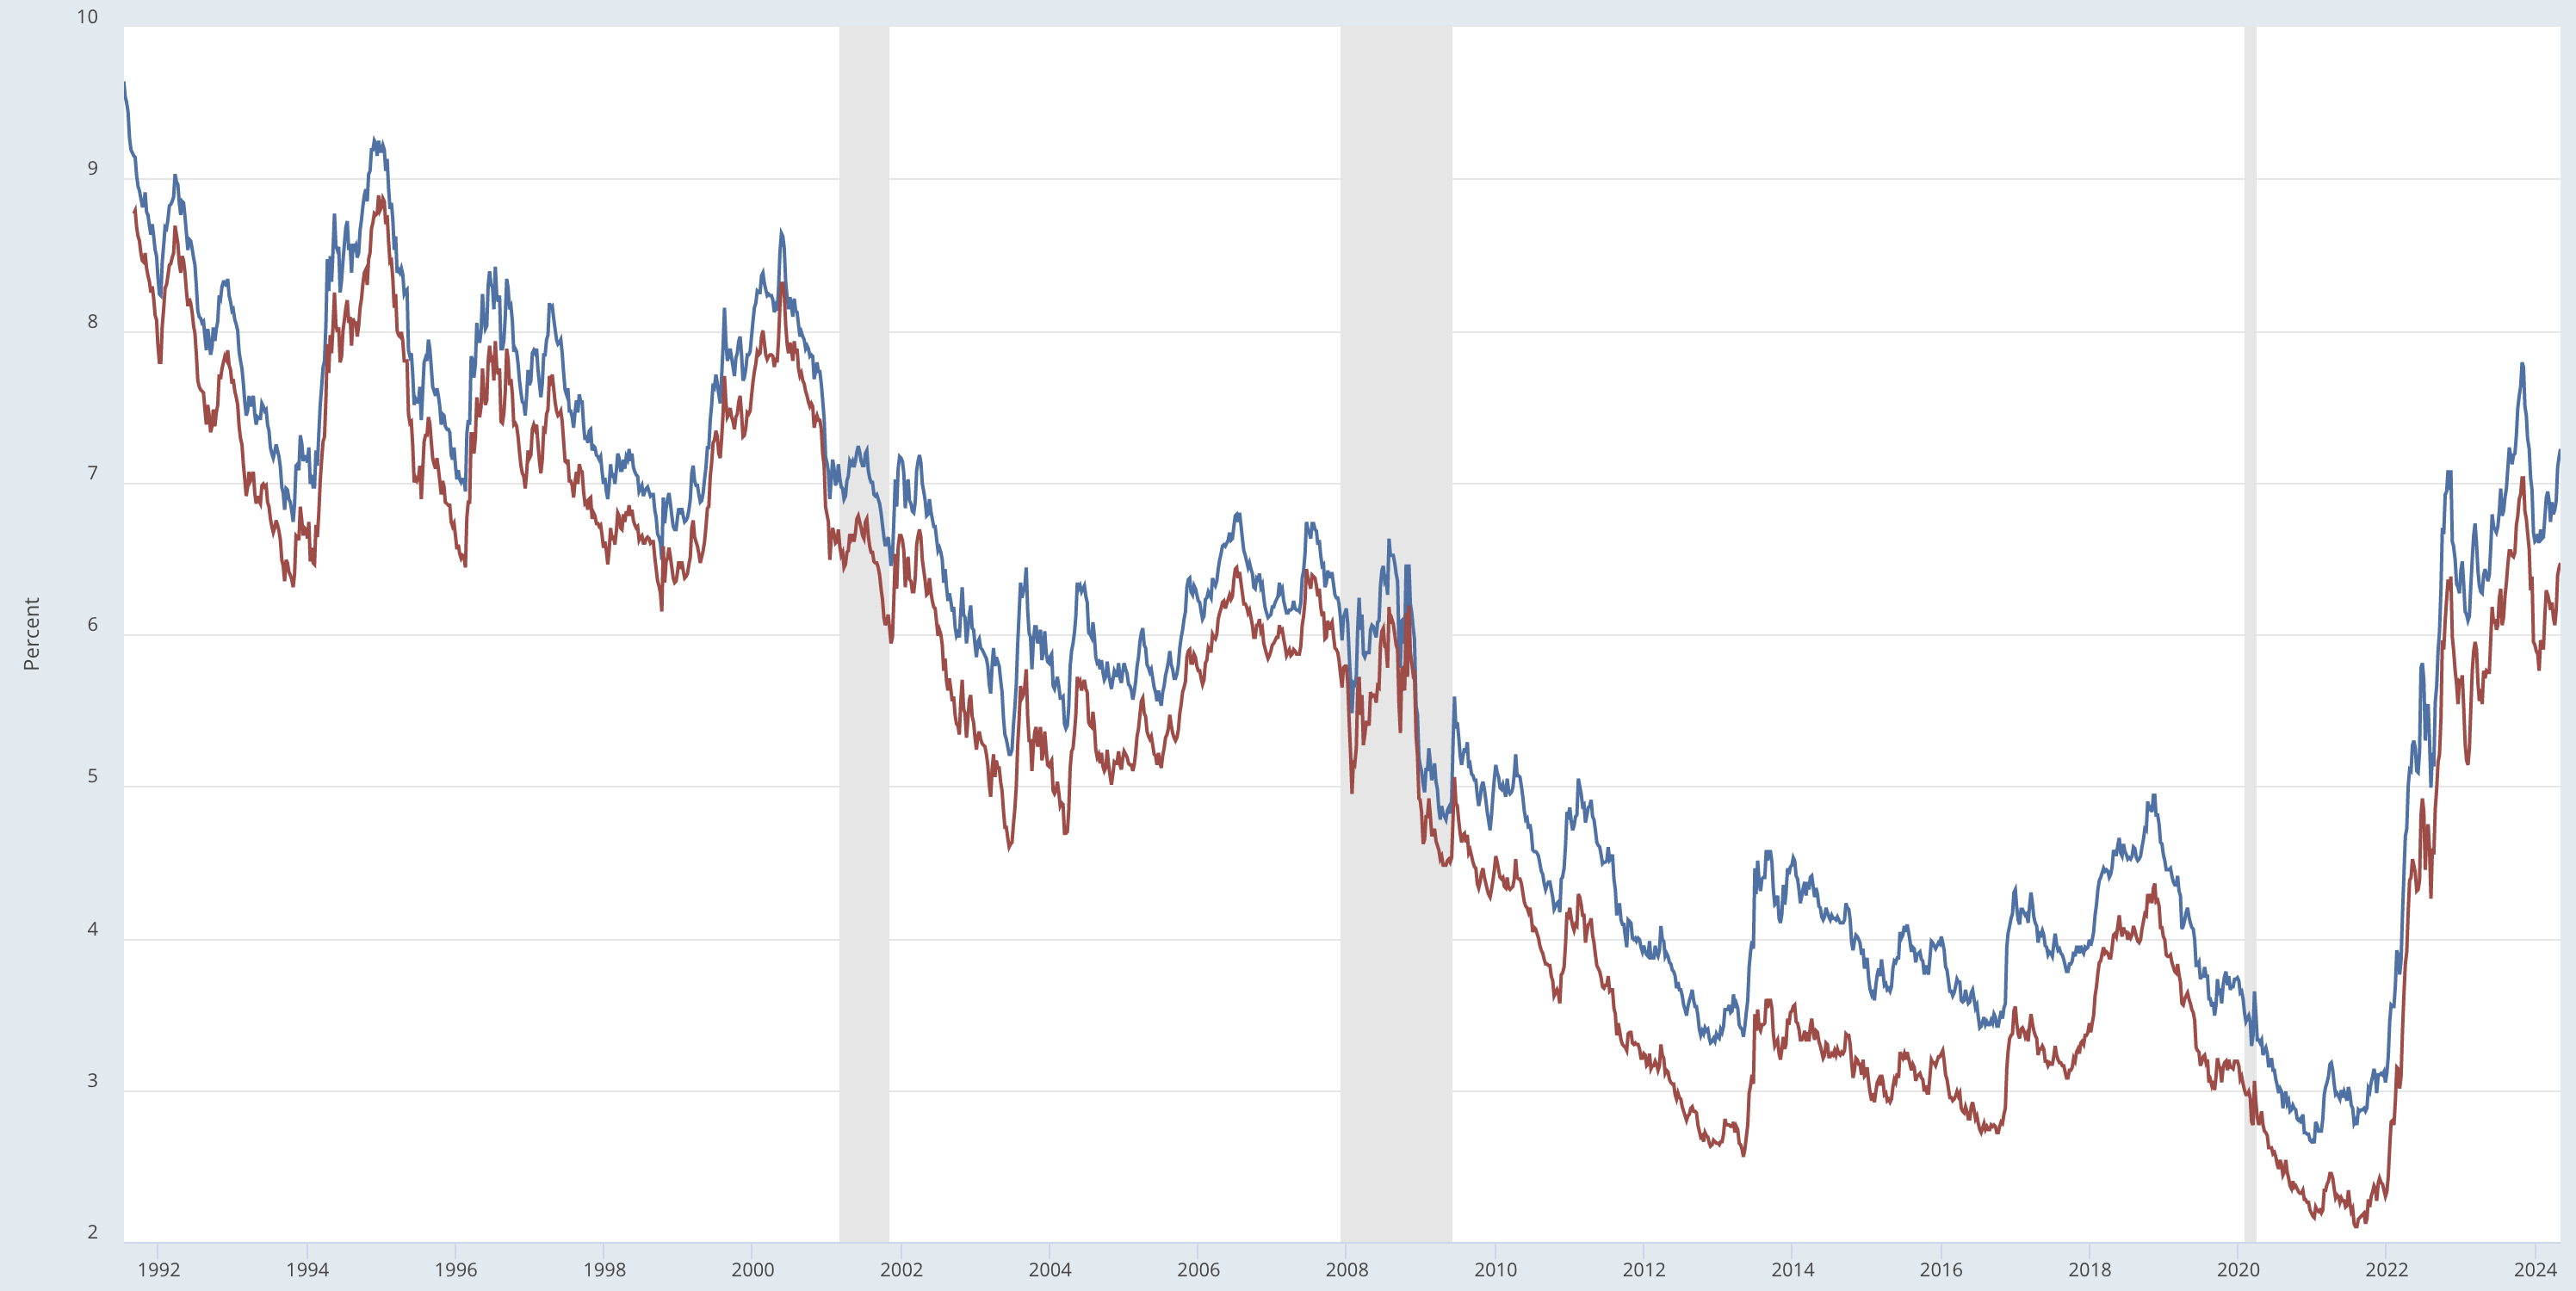
\includegraphics[scale=0.25]{img/mortgage.png}
        \caption{15-Year and 30-Year Fixed Rate Mortgage Average in the United States [FRED]} 
        \label{fig:mortgage}
      \end{figure}
    \end{example}

    There are countless loans, such as auto loans, home loans, student loans, bonds, etc. So how are these interest rates actually determined? To answer this, we must delve a little into macroeconomics. We will first talk about how banks work, the monetary policy, and the federal funds rate which then determines all other interest rates. 

  \subsection{Commercial Banks}

    With interest rates defined, we can get a general sense of how commercial banks work. The entire economy comes from the role of banks and the interest rates that is set upon them. There are many types of banks and many types of interest rates, which we will clarify. In any nation (we will use the U.S. as our primary example), we can divide all banks into the public, central bank and commercial, private banks. 

    \begin{definition}[Commercial/Retail Banks]
      A \textbf{commercial bank}, or \textbf{retail bank}, is what most people refer to as everyday banks. They provide basic banking services to individuals and to small/medium-sized businesses. These include
      \begin{enumerate}
        \item Accepting deposits and offering checking account services
        \item Making loans and mortgages
        \item Offering basic investment services such as CDs and safe deposit boxes
      \end{enumerate}
      Banks are businesses, too, and they make money in two ways:
      \begin{enumerate}
        \item They collect service charges and fees, ranging from account fees (maintenance charges, minimum balance, overdraft, etc.), safe deposit box fees, and late fees. 
        \item They earn money from interest they earn by lending out money to other clients. It is clear that the interest rate paid by the bank on the money they borrow is less than the rate charged on the money they lend (otherwise, they would not profit). 
      \end{enumerate}

      Because of the second reason, the majority of the deposits are not held by the bank. 

      \begin{figure}[H]
        \centering 
        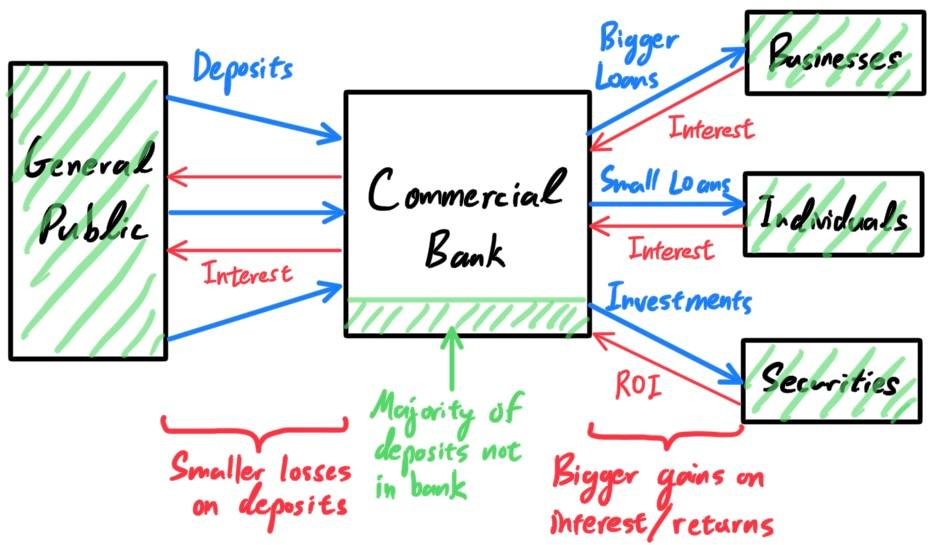
\includegraphics[scale=0.3]{img/Banks_Profit_on_Interest.jpg}
        \caption{Banks charge higher interest on loans than they pay on deposits to make a profit.}  
        \label{fig:Banks_Profit_on_Interest}
      \end{figure}
    \end{definition}

    Commercial banks are an important part of the economy because now only do they provide consumers with an essential service, they also help create capital and liquidity in the market.\footnote{Many banks now operate exclusively online, in contrast to their physical, \textit{brick-and-mortar} locations.} Indeed, they maintain the flow of money by taking money from customers deposit for their savings and lending it out to others. They play a role in the creation of credit, which leads to increase in production, employment, and consumer spending. 

    \subsubsection{Investment Banks}

      Investment banking provides financial services to companies within large and complex financial transactions. They focus mainly on company valuation to prepare for underwriting, M\&A, IPOs, and corporate reorganization. and they can be thought of as financial middlemen. 

      The separation between commercial and investment banking has been one of the primary features of the U.S. financial system since the 1930s. Congress is responsible for this separation, having decided that the investment banking activities of the nation's large commercial banks contributed to the widespread bank failures of the Depression. To prevent further failures, it passed legislation in 1935 called the Glass-Steagall Act that created a wall between commercial and investment banking activities and authorized a federal deposit insurance (FDIC) system. Investment banking, which involves dealings in stocks and bonds, was considered both risky and unsound for commercial banks that collected savings from the public.

      Since the Depression, a number of academic studies have suggested that such investment banking activities did not significantly contribute to massive bank failures. In addition, many now argue that the U.S. commercial banking system would actually be stronger if banking organizations were permitted to affiliate directly with investment banking concerns, a system usually referred to as universal banking. It turns out that the only major nations that require this is the U.S. and Japan, which was required to adopt this system after World War 2. Other large industrial countries like Germany and Switzerland have universal banking. The Glass-Steagall act was largely repealed in 1999, and since then most banks ahve engaged in both types of banking. 

      There are some benefits for banks that combine the functions of investment and commercial services. For example, a combination bank can use investment capabilities to aid a company in the sale of an IPO, and then use its commercial division to offer a generous line of credit to the new business. This enables the business to finance rapid growth and, consequently, to increase its stock price. A combination bank additionally gleans the benefits of increased trading, which brings in commission revenue.

      Many companies have separate banking divisions, but in order to know their structure, we should visit their history first. 

      \begin{example}[J.P. Morgan and Morgan Stanley]
        Pre-1935, the bank JP Morgan \& Co. was one of the largest banks in the U.S. within both commercial and investment banking. However, the Glass-Steagall Act forced JP Morgan \& Co. to choose to go into commercial banking (since investment banking was seen as risky post-depression). With this, J.P. Morgan made the decision to spin off its investment banking operations. Two JP Morgan partners, Henry S. Morgan and Harold Stanley, left to found their own investment bank, Morgan Stanley. In the years following the spin-off of Morgan Stanley, the securities business proved robust, while the parent firm was lagging behind. In 1959, JP Morgan merged with the Guaranty Trust Company to form the Morgan Guaranty Trust Company, boosting its stature. In 1970, Morgan Guaranty established a bank holding company called JP Morgan \& Co. Incorporated, but didn't do anything with it yet. In the 1980s, J.P. Morgan, along with other commercial banks, pushed for access to the investment banking industry, which was finally granted in 1989 by the Fed. The company migrated back to the J.P. Morgan brand, and to increase its presence, J.P. Morgan \& Co. merged with Chase Manhattan Bank to get J.P. Morgan Chase \& Co, making it one of the largest banks in the U.S. offering a full complement of investment banking, commercial banking, and retail banking (along with asset management, private banking, and private equity). Therefore, J.P. Morgan Chase Bank, or Chase bank, is the banking branch that constitutes the consumer and commercial banking subsidiary of J.P. Morgan Chase. 

        Morgan Stanley later merged with Dean Witter Discover \& Co., the spun-off financial services business of Sears, but later retained the name Morgan Stanley. While J.P. Morgan converted to a bank holding corporation in the 1980s to get into the investment banking industry, Morgan Stanley (and Goldman Sachs), the last two major investment banks in the U.S., both announced that they would become bank holding companies. Morgan Stanley has both investment banking and commercial banking services, along with other financial services. 
      \end{example}

      \begin{example}[Bank of America]
        Bank of America first originated in Italy, when Amadeo Pietro Giannini founded the Bank of Italy in San Francisco and merged it with Bank of America, Los Angeles (where he was a minority shareholder). The commercial bank expanded and acquired other companies around the nation, relabeled as the bank holding company BankAmerica with an investment banking division. However, following significant losses during the 1998 Russia bond default, NationsBank of Charlotte acquired BankAmerica in October 1998 for \$60 billion, taking the name Bank of America Corporation and still growing. In 2008, it acquired Merrill Lynch \& Co., and investment/wealth management company to become what it is now. BofA Securities (formerly BoA Merrill Lynch) is the investment banking subsidiary of BoA, and Merrill (formerly Merrill Lynch) is the investment/wealth management division of BoA. 
      \end{example}

  \subsection{Monetary Supply}

    How one keeps this money is important. We start off with the most liquid vs the least liquid. 

    \begin{definition}[Physical Currency]
      The \textbf{physical currency} represents banknotes and coins. This is clearly extremely liquid since if you physically have it, you can use it whenever you want. 
      \begin{figure}[H]
        \centering 
        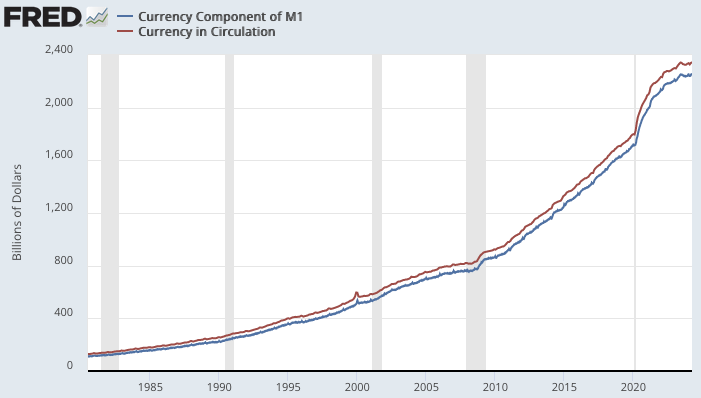
\includegraphics[scale=0.4]{img/currency_circulation.png}
        \caption{Currency in circulation} 
        \label{fig:circulation}
      \end{figure}
    \end{definition}

    \begin{definition}[Demand Deposits]
      \textbf{Demand deposits} refer to funds that can be withdrawn immediately at the holder's request without prior notice given to the bank. This is pretty much a checkings account. 
      \begin{figure}[H]
        \centering 
        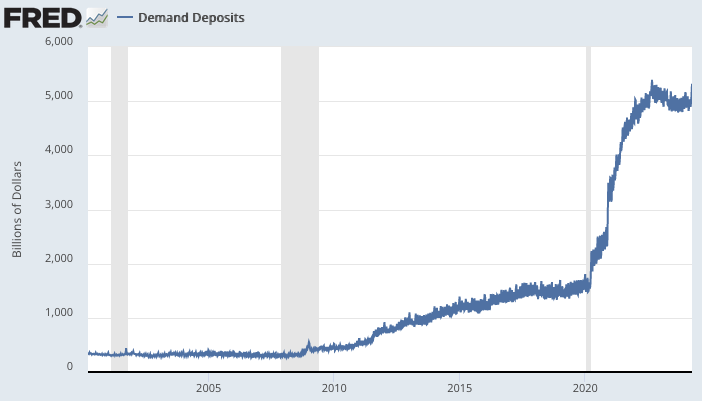
\includegraphics[scale=0.4]{img/demand_deposit.png}
        \caption{Demand deposits. } 
        \label{fig:demand_deposit}
      \end{figure}
    \end{definition}

    \begin{definition}[Savings Deposits]
      A \textbf{savings deposit} is less liquid than a checkings account since there are usually restrictions on how often you can withdraw from it. However, where this resides is a bit fuzzy, since savings accounts are also very liquid.\footnote{For example, at Bank of America you can withdraw up to 3 times without prior notice. }

    \end{definition}

    Since demand and savings deposits can be converted into real money in the near future, they are referred to as \textit{near money}. 

    \begin{definition}[Time/Term Deposits]
      \textbf{Time/Term deposits}, on the other hand, require the customer to lock in their money at a bank. This is further categorized into how long the term is (7 days to 2 years are considered \textit{short-term} and beyond are \textit{long-term}) and how big the deposit is (\$100k or more are considered large deposits). 
      \begin{figure}[H]
        \centering 
        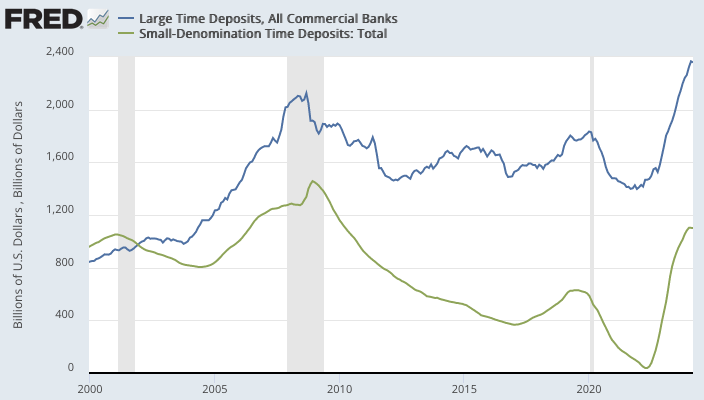
\includegraphics[scale=0.4]{img/time_deposits.png}
        \caption{Time deposits} 
        \label{fig:time_deposit}
      \end{figure}
    \end{definition}

    Term deposits are referred to as \textit{near, near money}. 

    \begin{definition}[Levels of Monetary Supply]
      In the U.S. (or any other nation), there is a certain amount of money flowing through the economy, known as the \textbf{monetary supply}. There are many subcategories of this, which we will elaborate now. 
      \begin{enumerate}
        \item \textbf{M0} is the total of all physical currency in public circulation and held by the public along with bank reserves\footnote{These are accounts at the central bank that can be exchanged for physical currency, which will be elaborated later}. 
        \item \textbf{M1} is M0 plus demand deposits and savings deposits. This is the most widely used metric of money supply. 
        \item \textbf{M2} is M1 plus short-term time deposits. 
        \item \textbf{M3} is M2 + large time deposits and \textit{money market funds}, which are funds that invest in short-term securities.\footnote{This is discontinued since 2006 by the fed since it provided no useful indicators. }
      \end{enumerate}
      You can see the monetary supply in the U.S., which are updated weekly. The M3 is updated quarterly. Since it consists of other assets that are less volatile, it is generally less volatile than M1. Note that prior to May 2020, savings accounts were not included in M1, but due to increased liquidity it is now included.
      \begin{figure}[H]
        \centering 
        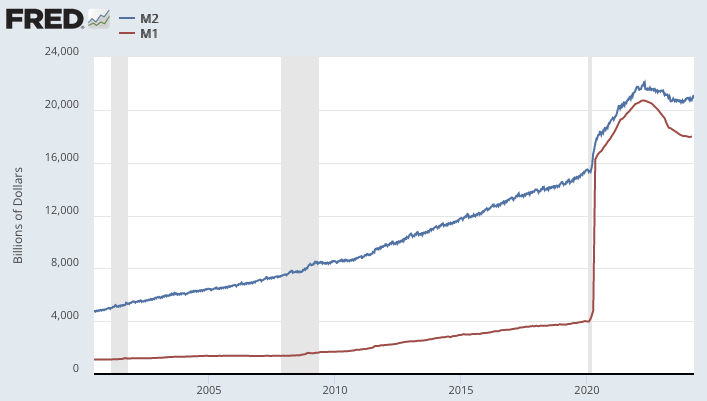
\includegraphics[scale=0.4]{img/Ms.png}
        \caption{M1 and M2 monetary supply. } 
        \label{fig:Ms}
      \end{figure}
    \end{definition}

    \begin{example}[U.S. Monthly Money Supply Measures]
      These are the money supply measures of the U.S. starting from May 2020, in billions of dollars. Note how they are consistently increasing. 
      \begin{center}
      \begin{tabular}{c|c|c}
        Date & M1 & M2 \\
        \hline
        May 2020 & 16,275.9&17,893.0\\
        Jun. 2020 & 16,601.7&18,179.6\\	
        Jul. 2020 & 16,792.6&18,320.0\\
        Aug. 2020 & 16,906.0&18,381.8\\
        Sep. 2020 & 17,176.3&18,605.0\\
        Oct. 2020 & 17,367.1&18,751.1\\
        Nov. 2020 & 17,610.0&18,960.2\\
        Dec. 2020 & 17,829.6&19,125.8\\
        Jan. 2021 & 18,109.6&19,378.7\\
        Feb. 2021 & 18,401.0&19,650.3\\
        Mar. 2021 & 18,682.9&19,896.2
      \end{tabular}
      \end{center}
    \end{example}

    \begin{definition}[Types of Money]
      There are actually different types of money: 
      \begin{enumerate}
        \item \textbf{Commodity money} is a medium of exchange that is an actual good, normally gold or silver, that had intrinsic value in other uses. These alternative uses gave commodity money value independent of its role as a medium of exchange. 

        \item \textbf{Commodity-backed money} is a medium of exchange with no intrinsic value, but whose ultimate value was guaranteed by a promise that it could always be converted into valuable goods on demand. For example, U.S. banks issued private paper bills, which promised to exchange their notes for gold and silver coins on demand. 
        
        This was preferred since it tied up fewer valuable resources. Although a note-issuing bank still had to keep some gold/silver on hand, it had to keep only enough to satisfy demands for redemption of its notes. It could rely on the fact that only a fraction of its paper notes would be redeemed on a normal day. 

        \item \textbf{Fiat money} is not even backed by any commodity. Rather, its value arises entirely from the fact that it is generally accepted as a means of payment, a role/policy that is decreed by the government (that is, it exists by government \textit{fiat}). This means that the "promise to pay" for commodity-backed money was replaced with the promise to accept that currency. 
      \end{enumerate}
    \end{definition}

  \subsection{Central Banks and Federal Funds Rate} 

    Note that we said that most of the money that banks receive are invested elsewhere. This can be risky since if a lot of people want to withdraw their money from the bank at once, the banks may not have enough liquidity to pay them back, leading to panic. This is known as a \textbf{bank run}. 

    \begin{definition}[Bank Runs, Failures]
      \textbf{Bank runs} happen when a large number of people, out of panic, start making withdrawals from banks because they feat the institutions will run out of money. A \textbf{bank panic} occurs when multiple banks endure runs at the same time. 
    \end{definition}

    \begin{definition}[FDIC Insurance]
      Customers find commercial bank investments, such as savings accounts and CDs, attractive because they are insured by the \textbf{Federal Deposit Insurance Corporation (FDIC)}, which is an independent federal agency insuring deposits in U.S. banks. This means that the FDIC insures deposits up to \$250,000 per depositor as long as the bank is a member firm of the FDIC. Therefore, people with more than \$250,000 should spread their savings out in multiple FDIC-insured banks, or across multiple accounts (a checking and multiple savings) in the same FDIC-insured bank. 
    \end{definition}

    In order to minimize the possibility of these bank runs, the government legally requires all banks operating in the U.S. to have a required \textbf{reserve ratio} (the amount of funds that a bank holds in reserve to ensure that it is able to meet liabilities in case of sudden withdrawals).\footnote{The \textit{International Banking Act of 1978} required branches of foreign banks operating in the U.S. to follow the same required reserve ratio standards.} These \textbf{federal funds} (the minimum amount required to have) are stored in the regional Federal Reserve banks (so the central bank acts as the banks' bank). Historically, these requirements are based on a percentage of the bank's total deposits (the total amount of money deposited into the bank).\footnote{The following requirements have been changed heavily especially after coronavirus. In fact, at March 2020, the minimum reserve requirement for all deposit institutions was fixed to 0\%.} 
    \begin{enumerate}
      \item 0\% requirement for banks with eligible deposits up to \$16 million. 
      \item 3\% requirement for banks up to \$122.3 million. 
      \item 10\% requirement for banks greater than \$122.3 million. 
    \end{enumerate}
    The end-of-the-day balances in each bank's account, averaged over two-week reserve maintenance periods, are used to determine whether the bank meets its reserve requirements. 

  
    \begin{figure}[H]
      \centering 
      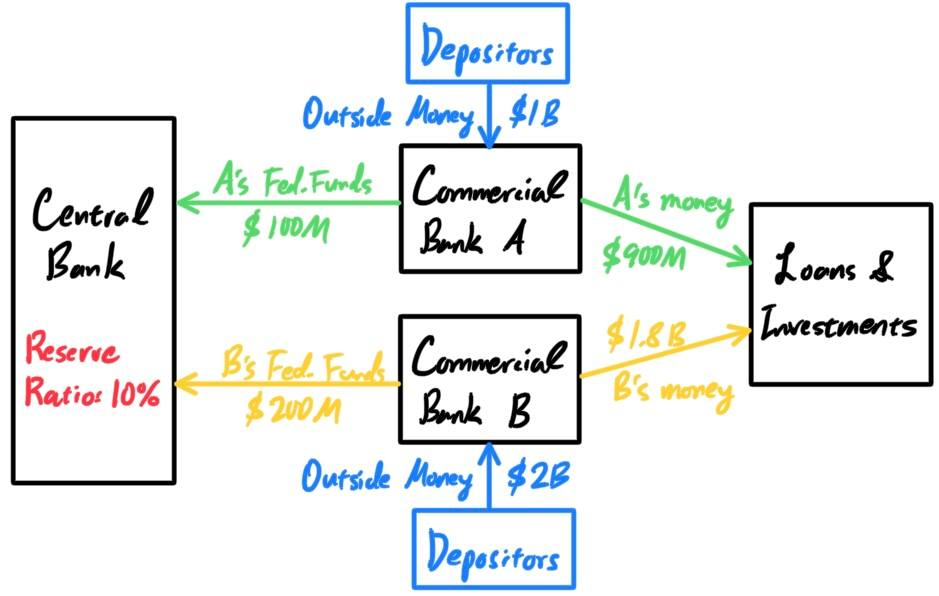
\includegraphics[scale=0.3]{img/Fed_Funds_Rate.jpg}
      \caption{If the reserve ratio is 10\%, commercial bank A must deposit \$100M in the Fed and can lend out \$900M. Bank B must deposit \$200M in the Fed and can lend out \$800M. } 
      \label{fig:Fed_Funds_Rate}
    \end{figure}

    But preventing bank runs isn't the only purpose of reserve requirements; it is used to influence the money supply in the economy. The higher the reserve requirements, the less money in circulation. The institution that controls this is the \textbf{central bank}. 

    \begin{definition}[Central Bank]
      A \textbf{central bank}, or \text{reserve bank} is an institution that manages the currency and monetary policy of a state and oversees their commercial banking system. Functions of a central bank include: 
      \begin{enumerate}
        \item \textbf{Monetary Policy}: by setting the official interest rate and controlling the money supply 
        \item \textbf{Financial Stability}: Acting as a government's banker and the bankers' bank ("lender of last resort") 
        \item \textbf{Reserve management}: Managing a country's foreign-exchange and gold reserves and government bonds
        \item \textbf{Banking Supervision}: Regulating and supervising the banking industry
        \item \textbf{Coins and Notes Issuance}
      \end{enumerate}
    \end{definition}

    \begin{definition}[Federal Reserve Structure]
      The \textbf{Federal Reserve}, or the \textbf{Fed}, is the central bank of the United States. The Fed is composed of several layers. 
      \begin{enumerate}
        \item It is governed by the 7-member presidentially appointed \textbf{Federal Reserve Board (FRB)}. 
        \item 12 regional Federal Reserve Banks, located throughout the nation (based in New York, Boston, Philadelphia, Cleveland, Richmond, Atlanta, Chicago, St. Louis, Minneapolis, Kansas City, Dallas, San Francisco), regulate and oversee privately owned commercial banks. 
        \item The \textbf{Federal Open Market Committee (FOMC)} sets the monetary policy, consisting of the FRB and the 12 regional bank presidents. 
      \end{enumerate}
      These banks protect regional economic interests. Even though they don't operator for profit, they generate income from interest on government securities acquired to Fed monetary policy actions. Unusually, it is a separate entity from the U.S. Department of the Treasury. 
    \end{definition}

    \begin{definition}[U.S. Department of the Treasury]
      The \textbf{Department of the Treasury (USDT)} is the national treasury of the Fed. Its purposes are listed: 
      \begin{enumerate}
        \item It oversees the \textbf{Bureau of Engraving and Printing} and the \textbf{U.S. Mint}, the two agencies responsible for printing all paper currency and coins. Note that some printing/minting does occur, but the vast majority of the American money supply is digitally debited and credited to major banks. 
        \item It executes money circulation in the fiscal system. 
        \item It collects all federal taxes through the Internal Revenue System (IRS). 
        \item It manages the U.S. government debt instruments (Treasury bonds). 
        \item It licenses and supervises banks. 
      \end{enumerate}
    \end{definition}

    The main difference between the central bank and other banks is that the central bank is \textit{not} a business, while the other banks are businesses, meaning that their purpose is the make money. The central bank's job is to control the economy and to prevent financial crises with the extra power they have as a part of the government (e.g. printing unlimited money, changing various rates). This power comes into the form of interest rates. 

    There is a dynamic relationship between the federal bank and the many commercial banks. They can lend money to each other, and depending on who lends who, different rates are charged. The two rates below are directly controlled by the Fed.

    \begin{definition}[Interest on Reserve Balances]
      The \textbf{interest rate on reserve balances (IORB)} is a combination of the \textbf{interest rate on required balances (IORR)} and \textbf{interest rate on excess reserves (IOER)}, which are the rates of interest that the central bank pays commercial banks on required reserves and excess reserves (i.e. the reserves held by a bank in excess of what is required, serving as a safety buffer). These are directly controlled by the Fed.
    \end{definition}

    \begin{definition}[Discount Rate]
      Going the other way, if commercial banks borrow money from the central bank, they must pay an interest. For example, banks can borrow funds to keep up their required reserves by taking a loan from the Fed itself at the discount rate. More specifically, there are actually three different discount rates: 
      \begin{enumerate}
        \item The \textbf{primary credit rate} (mentioned the most) is the basic interest rate charged to most banks (e.g. 0.25\%). 
        \item The \textbf{secondary credit rate} is charged to banks that don't meet the primary rate requirements. It is typically half a point higher than the primary credit rate (e.g. 0.75\%). 
        \item The \textbf{seasonal discount rate} is for small community banks that need a temporary boost in funds to meet local borrowing needs. This may include loans for farmers, students, resorts, and other seasonal activities. 
      \end{enumerate}
      This rate is directly controlled by the Fed. 
    \end{definition}

    Recognize that each bank wants to hold the optimal amount of federal funds. If it holds too few federal funds, it might not be able to honor its obligations to other banks (e.g., when they show up with checks written by its customers) or might fall below the legal amount of reserves it is required to hold. If it holds too many federal funds, it will earn less interest on its assets than it otherwise would on other investments. Hence, each bank is trying to hold the optimal amount of reserves, given its unique position and the opportunity cost of holding reserves. 

    \begin{definition}[Federal Funds Rate]
      So, there will inevitably be banks that hold too many federal funds that can lend money to banks that hold too few federal funds. Therefore, this money can be lent between banks, with the promise that those funds are paid back overnight. This financial market in which interbank lending occurs in the U.S. is called the \textbf{federal funds market}, and the interest rate the lending bank can charge is referred to as the \textbf{federal funds rate (FFR)}. There are two variations of this rate: 
      \begin{enumerate}
        \item The actual interest rate for a loan between two banks is determined through negotiations between them. The weighted average of this rate across all such transactions on a certain night is the \textbf{federal funds effective rate (FFER)}. 
        \item The \textbf{federal funds target rate (FFTR)} is a (usually quarter percent) range set by the FOMC (usually 8 times a year) as a guidepost, which they enforce by open market operations and adjustments in IOR/IOERs. The target rate is almost what is meant by the media referring to the Fed "changing interest rates." The actual FFR generally lies within the range of that target rate. 
      \end{enumerate}
    \end{definition}

    Note that the FFR is the benchmark interest rate of the economy, since all other interest rates on loans from commercial banks are dependent on it. That is, a higher FFR will mean that commercial banks will have to raise interest rates on all of their loans (to profit accordingly), and a lower FFR will mean that banks will lower their interest rates on loans. Therefore consumers should care about the FFR since it influences how much they pay to borrow and how much they're paid to save. 

    \begin{figure}[H]
      \centering 
      \includegraphics[scale=0.3]{img/3_Interest_Rates.jpg}
      \caption{The IOER is the interest on the flow of money from commercial banks to the central bank. The discount rate is the interest on the flow of money from the central bank to commercial banks. The fed funds rate is the interest on the flow of money between commercial banks.}
      \label{fig:3_Interest_Rates}
    \end{figure}

    \begin{theorem}[FFR]
      There are simple relationships between these rates. If I am a commercial bank that needs money to satisfy my overnight reserve requirements, then I can either borrow from the Fed (with the discount rate) or other commercial banks (with FFR). 
      \begin{enumerate}
        \item Since borrowing from the Fed with the fixed discount rate is always an option, other commercial banks should naturally have an FFR lower than the discount (EFFR<Discount).
        \item If I am a commercial bank that has extra money, then I can either loan it to the Fed at the IOER rate or other commercial banks at the FFR. The FFR should naturally be higher than the IOER (IOER<EFFR). 
      \end{enumerate}
      Combining these two gets 
      \begin{equation}
        \text{IOER} < \text{EFFR} < \text{Discount}
      \end{equation}
      Since the Fed has direct control over IOER and Discount, it has control over the FFR, which lies in between the two. 
    \end{theorem}

    \begin{example}[Recent Rates]
      We list some of the rates from May 2015 to now, with gaps of a few months in between (even though the rates change every month). 
      \begin{center}
      \begin{tabular}{r|l|l|l}
        Date & FFR& IOER & Discount Rate\\
        \hline
        05/01/2015 & 0.12\% & 0.25\% & 1\% \\
        11/01/2015 & 0.12\% & 0.25\% & 1\% \\
        12/01/2015 & 0.24\% & 0.37\% & 1\% \\
        02/01/2016 & 0.38\% & 0.5\% & 1\% \\
        10/01/2016 & 0.4\% & 0.5\% & 1\% \\
        01/01/2017 & 0.65\% & 0.75\% & 1\% \\
        04/01/2017 & 0.9\% & 1\% & 1.5\% \\
        08/01/2017 & 1.16\% & 1.25\% & 1.75\% \\
        01/01/2018 & 1.41\% & 1.5\% & 2\% \\
        04/01/2018 & 1.68\% & 1.75\% & 2.25\% \\
        08/01/2018 & 1.91\% & 1.95\% & 2.5\% \\
        10/01/2018 & 2.19\% & 2.2\% & 2.75\% \\
        03/01/2019 & 2.41\% & 2.4\% & 3\% \\
        07/01/2019 & 2.4\% & 2.35\% & 3\% \\
        11/01/2019 & 1.55\% & 1.55\% & 2.25\% \\
        04/01/2020 & 0.05\% & 0.1\% & 0.25\% 
      \end{tabular}
      \end{center}
      We can see that the inequalities generally hold, with the interest rates generally rising and falling together. This makes sense because the Fed would encourage commercial banks to borrow from each other rather than hold excess reserves, which is preferred over borrowing money directly from the Fed. But in extreme situations, the above inequality may not hold for brief periods. 
    \end{example}

    \begin{question}
      IOER has been actually greater than FFR consistently in the past 10 years. Why? Read \href{https://www.clevelandfed.org/publications/economic-commentary/2017/ec-201707-the-federal-funds-market-since-the-financial-crisis}{this}. 
    \end{question}

    Since the FFR is really the interest rate at the bottom of the chain, all other interest rates are essentially functions of the FFR.   

  \subsection{Monetary Policy}

    Now, we describe how the Fed uses these policies to control the monetary supply. We can interpret some sum of money "being" or "flowing" in the economy if it is available to use by commercial banks to invest in other securities, i.e., not in the federal funds. Also note that increasing the money in the economy allows commercial banks to have more cash reserves on hand, which induces them to lend them out at lower rates, making loans easier to get in the overnight market and thus decreasing the FFR. Keep in mind that
    \begin{align*} 
      \text{More money in economy} & \iff \text{FFR decreases}, \\
      \text{Less money in economy} & \iff \text{FFR increases}.
    \end{align*}

    Setting borrowing costs is how the Fed does its job; steering the world's largest economy between recession and overheating. They determine how "hot" the economy is by looking at various measures. The two most important ones are: 
    \begin{enumerate}
      \item Inflation, measured by the CPI/PPI, and usually targeted to be at 2\%. 
      \item Unemployment rate, measured by the CPS, which should be minimized. 
    \end{enumerate}
    The Fed controls this by changing the target FFR, which itself is controlled through open market operations. 

    \begin{definition}[Open Market Operations]
      The Fed can finally conduct \textbf{open market operations (OMO)}, which means to buy and sell government securities in the open market.
      \begin{enumerate}
        \item Buying government bonds (with possibly newly printed money) from a group of banks (or other entities in the market) $\rightarrow$ banks get more money by selling the bonds and thus more excess cash reserves, which they lend out in the fed funds market to other banks $\leftrightarrow$ FFR decreases. 
        \item Selling government bonds to banks (or other entities in the market) $\rightarrow$ banks lose money by buying the bonds $\rightarrow$ less money supply in commercial banks $\leftrightarrow$ FFR increases.
      \end{enumerate}
      As shown before, the federal funds rate may increase or decrease depending on the overall supply of reserves in the federal funds market. If the supply increases, this surplus of reserves pulls the FFR down, and if the supply decreases, this shortage of reserves pushes the FFR up; therefore, the federal funds rate acts as a catalyst that brings the federal funds market to equilibrium, ensuring that supply satisfies demand with the proper interest rate. 
      We can also categories OMOs as such: 
      \begin{enumerate}
          \item \textbf{Permanent Open Market Operations (POMOs)} refers to when the central bank actively buys and sells treasury securities in the open market on a continual basis. When any central bank \textit{consistently} uses the open market to buy/sell securities in order to adjust the money supply, it is engaging in POMOs. 
          \item \textbf{Temporary Open Market Operations} refers to when specific quantities of treasury securities are authorized to be purchased or sold for a period to address a financial crisis or other economic emergency. This is used to add or drain reserves available to the banking system on a temporary basis. 
      \end{enumerate}
    \end{definition}

    We have already seen how the Fed uses open market operations to adjust the FFR. But how does this exactly affect other rates? In the simplest terms, 
    \begin{enumerate}
      \item A decreased FFR means that banks can borrow money easily at low interest rates, meaning that they can then use the reserves that they have obtained at lower rates to offer loans at lower interest rates to consumers/businesses. The cheaper credit in turn causes consumers/businesses to spend and invest, boosting sales and economic activity (an \textbf{expansionary goal}). 
      
      Furthermore, an decreased FFR, which implies lower yields, tend to push away investment capital from investors abroad seeking higher returns on bonds and interest-rate products. This makes the U.S. dollar weaker. 
      
      \item An increased FFR means that banks borrow less money due to higher interest rates, meaning that they give loans at even higher ones to consumers. This increase in the cost of credit through the funds rate curbs demand and reduces consumers/firms taking out loans to spend and invest, leading to an economic cooldown (a \textbf{contractionary goal}). 
      
      Furthermore, an increased FFR, which implies higher yields, tend to attract investment capital from investors abroad seeking higher returns on bonds and interest-rate products. This makes the U.S. dollar stronger. 
    \end{enumerate}

    Note that the FFR is the \textit{benchmark interest rate} of the economy, since all other interest rates on loans from commercial banks are dependent on it. That is, a higher FFR will mean that commercial banks will have to raise interest rates on all of their loans (to profit accordingly), and a lower FFR will mean that banks will lower their interest rates on loans. Therefore consumers should care about the FFR since it influences how much they pay to borrow and how much they're paid to save. 

    Let's talk about what aspects of the economy the FFR affects: 
    \begin{enumerate}
      \item Bond market. Remember that when interest rates rise, bond prices generally fall (in the secondary market), and when interest rates fall, bond prices generally rise. However, in the primary market, how does the original coupon rate get established? 
      
      \item \textbf{Prime Rates}, or the \textbf{Bank Prime Loan Rate}, is the credit rate that banks extend to their most credit-worthy customers, leading to a rise in every other interest rate. Since the FFR determines the minimum interest rate that banks must put on a loan to make a profit, it is clear that 
      \[\text{Increased Fed funds rate } \implies \text{ Increased prime rate}\]
      In fact, prime rates are pegged at 300 points (3\%) over the target rate. Since prime rates represent the base rate at which banks loan out to consumers, an increase in this base rate will increase every other rate, such as 
      \begin{enumerate}
          \item Adjustable-rate mortgages
          \item Auto loans
          \item Variable-rate credit card expenses
          \item CDs, savings accounts, and money market accounts
      \end{enumerate}
      depending on factors such as one's assets, liabilities, and creditworthiness. 
      \item If global capital flows are moving into dollar-denominated assets, chasing higher rates of return, the U.S. dollar strengthens, causing it to be more expensive in the exchange rate. 
      \item \textbf{Exports}: Due to the dollar strength, U.S. export sales may decline since foreign countries will need to pay more for U.S. goods. 
      \item \textbf{Imports, Inflation:} A strong dollar makes foreign imports cheaper, since the price of foreign currency is relatively cheap. This results in cheaper products at U.S. stores (since domestic companies have to keep prices low to compete with cheap foreign imports), and these low prices translate to low inflation. 
    \end{enumerate}
    On the extreme end, zero and negative rate environments benefit the economy through easier borrowing. In an extreme negative rate environment, borrowers even receive interest payments. 

    \begin{definition}[Other Monetary Policy Tools]
      Most of the time, the Fed funds rate is unchanged or changed incrementally by 0.25\%, but in extreme cases, the rate can change drastically. However, in less extreme cases, the Fed can also adjust these rates too to influence monetary policy. 
      \begin{enumerate}
        \item \textit{It can change the bank reserve requirements.} If they are higher, more money is "locked in" the required reserve and the money supply shrinks. If they are lower, more money moves from the required reserve to the excess reserve, allowing better trading rates. 
        \item \textit{It can change the discount rates.} If the discount rates are higher, it will discourage commercial banks from loaning money from the Fed, and if rates are lower, commercial banks have more of an incentive to loan money from central banks. 
        \item \textit{It can change the IOR/IOER}. If the IOER rate is low, banks would prefer to lend funds out since it will be more profitable to gain interest according to the FFR rather than the IOER. This increases cash circulation and makes it easier to borrow money. If the IOER rate is high, then banks would prefer to keep more money at the Fed rather than lend to a potentially risky borrower. This chokes the circulation of money since banks won't want to take money out of their excess reserves. 
      \end{enumerate}
    \end{definition}

  \subsection{Money Multiplier Effect}

    Recall that the $M0$ monetary supply, or the monetary base, is the total amount of money that the Fed has injected into the U.S. economy. For this reason, the monetary base is also called \textbf{high-powered money}. However, the $M1$ and $M2$ supplies are usually much larger than the $M0$. As of 2021, the $M0$ supply is USD 6.4T, while the $M1$ is USD 20.6T and $M2$ is 21.6T. Where did this extra money come from? The \textbf{multiplier effect}, which exists in the \textbf{fractional reserve banking system}, tells us that infusions of capital will have a broad snowball effect on various aspects of economic activity. That is, if the government injects a certain amount of money into the economy, it turns out that the money supply increases by multiple factors of what was put in.

    \begin{example}[The Credit Market Funnel]
      Suppose that the government prints USD 10B and credits an additional USD 90B (i.e., credits loans by selling bonds) to banks and other depository institutions. At first, it might seem like the economy just received a monetary influx of USD 100B, but that is actually a very small percentage of the actual money creation. Let us assume that the reserve requirement is 10\% (that is, all depository institutions must have 10\% of their deposits kept in the federal reserve).

      \begin{enumerate}
        \item The banks get USD 100B. With the 10\% requirement, they must keep 10B in reserves and can lend out 90B in investments or loans, which goes into the hand of institutions and individuals. There is a total of 100B in money supply: 90B lent out and 10B in reserves.
        \item These institutions/individuals will deposit the 90B receivings in banks. The banks get USD 90B. With the 10\% requirement, they must keep 9B in reserves and can lend out 81B in investments or loans, which goes into the hand of institutions and individuals. There is a total of 190B in money supply: 90+81=171B lent out and 10+9=19B in reserves.
        \item These institutions/individuals will deposit the 81B receivings in banks. The banks get USD 81B. With the 10\% requirement, they must keep 8.1B in reserves and can lend out 72.9B in investments or loans, which goes into the hand of institutions and individuals. There is a total of 271B in money supply: 90+81+72.9=243.9B lent out and 10+9+8.1=27.1B in reserves.
        \item These institutions/individuals will deposit the 72.9B receivings in banks. The banks get 72.9B USD...
      \end{enumerate}

      Calculations for the first few deposit/lending cycle is shown. Note that money supply is all of the amount lent out until now plus all the reserves accumulated until now.

      \begin{tabular}{|l|l|l|l|l|l|}
        \hline
        Bank & Deposit Amount & Amount Lent Out & Money Supply & Reserves & Total Reserves \\
        \hline
        1 & \$100.00 & \$90.00 & \$100.00 & \$10.00 & \$10.00 \\
        2 & \$90.00 & \$81.00 & \$190.00 & \$9.00 & \$19.00 \\
        3 & \$81.00 & \$72.90 & \$271.00 & \$8.10 & \$27.10 \\
        4 & \$72.90 & \$65.61 & \$343.90 & \$7.29 & \$34.39 \\
        5 & \$65.61 & \$59.05 & \$409.51 & \$6.56 & \$40.95 \\
        6 & \$59.05 & \$53.14 & \$468.56 & \$5.90 & \$46.86 \\
        7 & \$53.14 & \$47.83 & \$521.70 & \$5.31 & \$52.17 \\
        \ldots & \ldots & \ldots & \ldots & \ldots & \ldots \\
        \hline
      \end{tabular}

      This continues on in the form of a geometric series with a common ratio of 0.9 (1 minus the reserve ratio of 10\%). After an infinite time, the total money supply converges 10 times USD 100B to become USD 1 trillion.
    \end{example}

    \begin{definition}[Money Multiplier Effect]
      When the central bank creates monetary reserves and sends those to commercial banks, banks can lend much of that money to consumers, who will also deposit most into other banks. 
    \end{definition}

    One subtle distinction that we must mention is that in the ideal case where banks loan out precisely 90\% of their deposits and the economy deposits 100\% of their savings, this multiplier is actually called the \textbf{deposit multiplier}. It is indeed the case that the reserve requirement is about 10\%, but the $M1/M2$ supplies are not even close to 10 times the $M0$ supply. This is because of imperfections due to excess reserves, savings, and conversions to cash by consumers, the actual multiplier, called the \textbf{money multiplier}, is ultimately less. Borrowers do not spend all of the money received from bank loans. If they did, and if banks loaned out every possible dollar beyond the minimum reserve requirements, then the deposit multiplier and the money multiplier would be close to exactly equivalent.

\section{Fiscal Policy}

  \subsection{Federal Income and Spending}

    The government has two jobs: 
    \begin{enumerate}
      \item Spend money effectively 
      \item Don't spend too much. 
    \end{enumerate}

    In order to understand what the government does, we should look at the U.S.'s federal income and spending, in which the budget is planned out thoroughly every fiscal year. To create the budget plan, the president initiates budget negotiations by submitting a budget to Congress for the subsequent fiscal year by February. It should have predictions for U.S. tax revenue and estimated budget requirements. Congress responds with spending appropriation bills that go to the president by June 30. If both houses do not pass the budget, the budget resolutions from previous years carry over. The House or Senate may also propose their budget resolutions independently of the White House. 

    \begin{example}[2021 Biden Stimulus Package]
      In May 2021, President Biden proposed a \$6 trillion budget aimed at an economic agenda that includes large new investments in education, transportation, and fighting climate change. It also predicts total spending to rise to \$8.2 trillion by 2031.
    \end{example}

    \begin{definition}[Federal Spending Targets]
      The federal spending targets are: 
      \begin{enumerate}
        \item \textbf{Discretionary Spending}: Portion of the budget that is decided by Congresss each year through an appropriations process. \textit{(Military, Education, Health, Veteran's Benefits, Government, Housing \& Community, Transportation, International Affairs, Foreign Aid/Loans, Energy \& Environment, Labor, Science, Food \& Agriculture)}
        \item \textbf{Mandatory Spending}: All spending that does not take place through appropriations legislation. (\textit{Social Security}, Unemployment, Labor, Medicare \& Health (mainly), Education, Government, Food \& Agriculture, Veteran's Benefits, Transportation, Housing \& Community, Infrastructure)
        \item \textbf{(Net) Interest on Debt}: All interest payments the federal government makes on accumulated debt, minus interest income received by the government. Usually the net interest is a spending, not income.
      \end{enumerate}
    \end{definition}

    We use statistics from \href{https://datalab.usaspending.gov/americas-finance-guide/spending/categories/}{2021}.
    Mandatory progams include:
    \begin{enumerate}
      \item \textbf{Income Security (\$1.6T)}: Disability assistance, food and nutrition assistance, supplemental security income (income for disabled), tax credits, unemployment compensation, housing assitance
      \item \textbf{Social Security (\$1.1T)} is the commonly used term for the OASDI program, which provides benefits for three broad categories of individuals: retirees, disabled, and survivors, along with other beneficiaries such as spouses, divorced, orphans, widows, etc. The average monthly Social Security benefit for December 2019 was \$1,382, with 65 million individuals receiving benefits as of 2020. They are funded primarily through payroll taxes.
      \item \textbf{Healthcare (\$797B)}, such as \textbf{Medicaid} provides health insurance for low-income individuals.
      \item \textbf{Medicare (\$697B)} primarily provides health insurance for the elderly and for some disabled younger individuals.
      \item \textbf{Veterans Benefits (\$234B)}: Income security for veterans and healthcare assistance.
      \item \textbf{Agriculture (\$50B)}: Agricultural Research \& Services, Farm Income Stabilization
      \item \textbf{International Affairs (\$47B)}: Foreign Aid, Poverty, Disease Prevention \& Control, Diplomacy programs, foreign military aid, United Nations programs, Food
    \end{enumerate}
    Discretionary programs include:
    \begin{enumerate}
      \item \textbf{Defense (\$755B)}: Power Projections (sea \& air power), munitions (maintenance \& procurement of ammunition inventory), nuclear deterrence, missile defense, space systems, cyberspace operations, overseas contingency operations (funds available for unexpected warfare abroad).
      \item \textbf{Transportation (\$155B)}: Road improvements and repairs, air traffic control, railroad \& infrastructure investments.
      \item \textbf{Education (\$263B)}: K-12 education grants, school choice programs, disability \& special education programs, lunch assistance, No Child Left Behind Program (offering provisions to disadvantaged students), IDEA Special Education State Grants (for education of disabled), child nutrition programs, higher education
      \item \textbf{Administration of Justice (\$72B)}: Federal Law Enforcement, Litigative, Judicial Activities, Criminal Justice Assistance, Correctional Activities
      \item \textbf{General Science, Space, Technology (\$35.6B)}: Space Flight, research, general science \& basic research
    \end{enumerate}

    \begin{definition}[Federal Income Sources]
      The federal spending targets are: 
      \begin{enumerate}
        \item \textbf{Taxes}: Income tax, payroll tax, corporate tax, excise tax, tariffs on imports, estates tax.
        \item \textbf{One-time Payments}: Fines, etc.
      \end{enumerate}
    \end{definition}

  \subsection{Budget Deficits}

    Historical data on U.S. income and spending reveals that the government almost always spends more than it earns, i.e. has a deficit. The dollar amount of national debt is not as important as its \textbf{debt-to-GDP ratio}, since a bigger economy translates to more revenue for a government to pay off debts.

    \begin{figure}[H]
      \centering 
      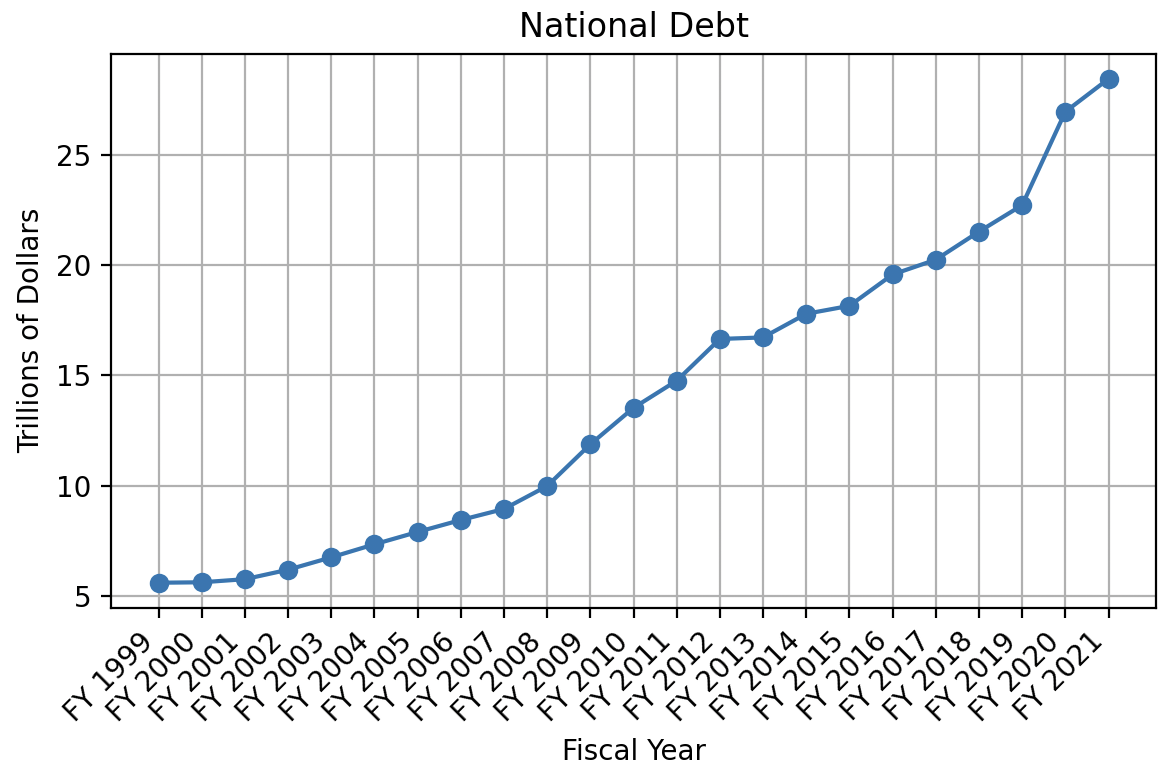
\includegraphics[scale=0.6]{img/national_debt.png}
      \caption{} 
      \label{fig:national_debt}
    \end{figure}

    \begin{figure}[H]
      \centering 
      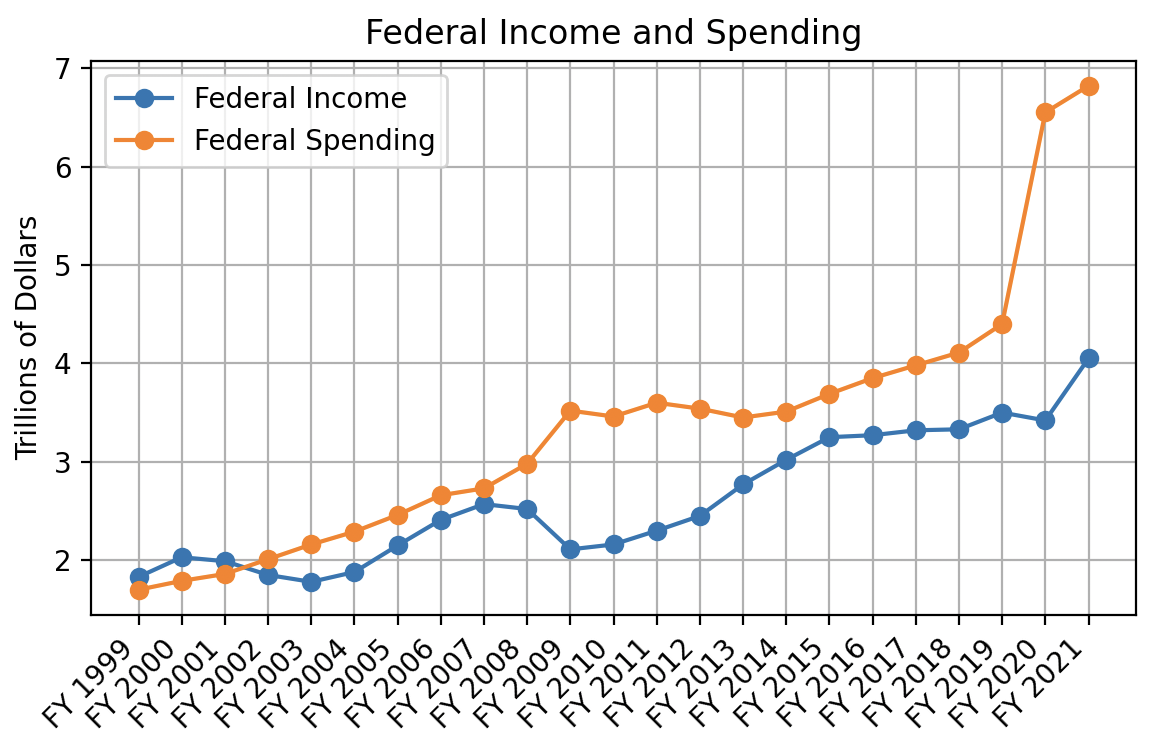
\includegraphics[scale=0.6]{img/income_spending.png}
      \caption{} 
      \label{fig:income_spending}
    \end{figure}

    \begin{table}[H]
      \begin{tabular}{|l|l|l|l|l|l|l|}
      \hline
      & GDP & Federal Income & Federal Spending & Deficit/Surplus & National Debt & Debt Added \\ \hline
      FY 2021 & \$22.40T & \$4.05T (18.1\%) & \$6.82T (30.5\%) & -\$2.77T (12.4\%) & \$28.43T (125.2\%) & \$1.49T \\ \hline
      FY 2020 & \$20.70T & \$3.42T (16.3\%) & \$6.55T (31.3\%) & -\$3.13T (15.0\%) & \$26.94T (130.1\%) & \$4.23T \\ \hline
      FY 2019 & \$21.10T & \$3.50T (16.3\%) & \$4.40T (21.0\%) & -\$984B (4.6\%) & \$22.71T (107.6\%) & \$1.20T \\ \hline
      FY 2018 & \$20.24T & \$3.33T (16.5\%) & \$4.11T (20.3\%) & -\$779B (3.8\%) & \$21.51T (106.3\%) & \$1.27T \\ \hline
      FY 2017 & \$19.18T & \$3.32T (17.3\%) & \$3.98T (20.8\%) & -\$665B (3.5\%) & \$20.24T (105.5\%) & \$670B \\ \hline
      FY 2016 & \$18.41T & \$3.27T (17.8\%) & \$3.85T (20.9\%) & -\$585B (3.2\%) & \$19.57T (106.3\%) & \$1.42T \\ \hline
      FY 2015 & \$17.90T & \$3.25T (18.2\%) & \$3.69T (20.6\%) & -\$439B (2.45\%) & \$18.15T (101.4\%) & \$360B \\ \hline
      FY 2014 & \$17.79T & \$3.02T (17.5\%) & \$3.51T (20.3\%) & -\$485B (2.8\%) & \$17.79T (103.2\%) & \$1.07T \\ \hline
      FY 2013 & \$16.58T & \$2.77T (16.7\%) & \$3.45T (20.8\%) & -\$680B (5.5\%) & \$16.72T (100.8\%) & \$70B \\ \hline
      FY 2012 & \$16.03T & \$2.45T (15.3\%) & \$3.54T (22.1\%) & -\$1.09T (6.8\%) & \$16.65T (105.3\%) & \$1.89T \\ \hline
      FY 2011 & \$15.38T & \$2.30T (15.0\%) & \$3.60T (23.4\%) & -\$1.30T (8.5\%) & \$14.76T (96.0\%) & \$1.23T \\ \hline
      FY 2010 & \$14.80T & \$2.16T (14.6\%) & \$3.46T (23.4\%) & -\$1.29T (8.7\%) & \$13.53T (91.4\%) & \$1.65T \\ \hline
      FY 2009 & \$14.42T & \$2.11T (14.6\%) & \$3.52T (24.4\%) & -\$1.41T (9.8\%) & \$11.88T (82.4\%) & \$1.89T \\ \hline
      FY 2008 & \$14.75T & \$2.52T (20.2\%) & \$2.98T (20.2\%) & -\$459B (3.1\%) & \$9.99T (67.6\%) & \$1.04T \\ \hline
      FY 2007 & \$14.32T & \$2.57T (17.9\%) & \$2.73T (19.1\%) & -\$161B (1.1\%) & \$8.95T (62.5\%) & \$500B \\ \hline
      FY 2006 & \$13.69T & \$2.41T (17.6\%) & \$2.66T (19.4\%) & -\$248B (1.8\%) & \$8.45T (61.8\%) & \$540B \\ \hline
      FY 2005 & \$12.89T & \$2.15T (16.7\%) & \$2.46T (19.2\%) & -\$318B (2.5\%) & \$7.91T (61.3\%) & \$560B \\ \hline
      FY 2004 & \$12.09T & \$1.88T (15.6\%) & \$2.29T (19.0\%) & -\$412B (3.4\%) & \$7.35T (60.8\%) & \$590B \\ \hline
      FY 2003 & \$11.33T & \$1.78T (15.7\%) & \$2.16T (19.1\%) & -\$375B (3.3\%) & \$6.76T (59.7\%) & \$560B \\ \hline
      FY 2002 & \$10.88T & \$1.85T (17.0\%) & \$2.01T (18.5\%) & -\$158B (1.5\%) & \$6.20T (57.0\%) & \$430B \\ \hline
      FY 2001 & \$10.57T & \$1.99T (18.8\%) & \$1.86T (17.6\%) & +\$128B (1.2\%) & \$5.77T (54.6\%) & \$140B \\ \hline
      FY 2000 & \$10.15T & \$2.03T (20.0\%) & \$1.79T (17.6\%) & +\$236B (2.3\%) & \$5.63T (55.5\%) & \$20B \\ \hline
      FY 1999 & \$9.51T & \$1.83T (19.2\%) & \$1.70T (17.9\%) & +\$126B (1.3\%) & \$5.61T (58.9\%) & \$130B \\ \hline
      \end{tabular}
    \end{table}

    Some points to make:

    \begin{enumerate}
      \item The ridiculous spike in Federal spending in 2020 and 2021 was due to coronavirus.
    \end{enumerate}

    A nation can reduce its debt in one of five ways. All of them are basically ways to save/raise money and to decrease the federal deficit. 
    \begin{enumerate}
      \item \textbf{Increase Income} by increasing taxes
      \item \textbf{Sell Debt} by selling government bonds.  
      \item \textbf{Reduce Spending} by cutting costs on projects
      \item \textbf{Debt Restructuring}: Countries would move their debt from the private sector to public sector that might be better handle the impact of a country's default. Bondholders can also agree to accept a reduced percentage of what they are owed, along with the maturity dates of bonds being extended.
      \item \textbf{Monetization of Debt} by printing more money, which may lead to dangerous levels of inflation.
      \item \textbf{Outright Default} which would be destructive and affect the credit-worthiness of the U.S.
    \end{enumerate}

  \subsection{Taxation}

    We begin with the most straightforward way. 

    \begin{definition}[Taxes]
      To help fund public works and services, and to build and maintain the infrastructures used in a country, the government taxes its individual and corporate residents. Most governments use an agency or department to collect taxes; in the U.S. this is performed by the \textbf{Internal Revenue Service (IRS)}. There are several very common types of taxes: 
      \begin{enumerate}
        \item \textbf{Income Tax} - A percentage of individual earnings filed to the federal government
        \item \textbf{Corporate Tax} - A percentage of corporate profits taken as tax by the government
        \item \textbf{Sales Tax} - Taxes levied on certain goods and services
        \item \textbf{Property Tax} - Taxes based on the value of land and property assets
        \item \textbf{Tariffs} - Taxes on imported goods
        \item \textbf{Estate Tax} - Rate applied to the fair market value of property in a person's estate at the time of death
        \item \textbf{Capital Gains Taxes} - Taxes on income that results from the sale of assets in which the sale price was higher than the purchasing price 
      \end{enumerate}
      The \textbf{tax rate} (i.e. the percentage at which an individual/corporation is taxed) can differ widely depending on the type of tax and the country. These taxes are filed as: 
      \begin{enumerate}
        \item Single
        \item Head of Household
        \item Married, filing jointly
        \item Married, filing separately 
      \end{enumerate}
    \end{definition}

    \begin{definition}[Progressive, Regressive Tax System]
      Like many nations, the U.S. has a \textbf{progressive tax system}, through which a higher percentage of tax revenues are collected from high-income individuals/corporations rather rather than from low-income individual earners (as done in a \textbf{regressive tax system}). Taxes are imposed at the federal, state, and local levels. Generally, 
      \begin{enumerate}
        \item the federal government levies income, corporate, and payroll taxes
        \item the state levies sales taxes
        \item municipalities or other local governments levy property taxes
      \end{enumerate}
    \end{definition}

    \begin{example}[2020 U.S. Tax Brackets]
      There are seven federal tax brackets for the 2020 tax year. For single filers, we have
      \begin{center}
      \begin{tabular}{c|c|c}
        Tax Rate & Taxable Income Bracket & Tax Owed \\
        \hline
        10 \% & \$0 to \$9,875 & 10\% of taxable income \\
        12\% & \$9876 to \$40,125 & \$987.50 plus 12\% of amount over \$9,875\\
        22\% & \$40,126 to \$85,525 & \$4,617.50 plus 22\% of amount over \$40,125\\
        24\% & \$85,526 to \$163,300 & \$14,605.50 plus 24\% of amount over \$85,525\\
        32\% & \$163,301 to \$207,350 & \$33,271.50 plus 32\% of amount over \$163,300\\
        35\% & \$207,351 to \$518,400 & \$47,367.50 plus 35\% of amount over \$207,350\\
        37\% & \$518,401 or more & \$156,235 plus 37\% of amount over \$518,400
      \end{tabular}
      \end{center}
      Note that you don't lose anything by moving up a tax bracket. That is, if you earn \$520,000, then the 37\% tax does not apply to the entire \$520,000. You get taxed 10\% of the first \$9,875, then 12\% of your income past \$9,876 up to \$40,125, and so on. 

      However, if you are married, you can file jointly. This means that if the husband is only working and the wife is unemployed, then the husband has an advantage in tax benefits since the overhead for every income bracket is increased (in fact, doubled until the 6th bracket). For married pairs, filing jointly, we have 
      \begin{center}
      \begin{tabular}{c|c|c}
        Tax Rate & Taxable Income Bracket & Tax Owed \\
        \hline
        10 \% & \$0 to \$19,750 & 10\% of taxable income \\
        12\% & \$19,751 to \$80,250 & \$1,975 plus 12\% of amount over \$19,750\\
        22\% & \$80,251 to \$171,050 & \$9,325 plus 22\% of amount over \$80,250\\
        24\% & \$171,051 to \$326,600 & \$29,211 plus 24\% of amount over \$171,050\\
        32\% & \$326,601 to \$414,700 & \$66,543 plus 32\% of amount over \$326,600\\
        35\% & \$414,701 to \$622,050 & \$94,735 plus 35\% of amount over \$414,700\\
        37\% & \$622,051 or more & \$167,307.50 plus 37\% of amount over \$622,050
      \end{tabular}
      \end{center}
    \end{example}

    \begin{example}[2020 Sales Taxes by State]
      Since the state levies sales taxes, we list them for some states. 
      \begin{center}
      \begin{tabular}{l|l}
          State & Sales Rate \\
          \hline
          Alabama & 4.00\% \\
          California & 7.25\% \\
          Washington D.C. & 6.00\% \\
          Florida & 6.00\% \\
          Illinois & 6.25 \%\\
          Indiana & 7.00\%\\
          Massachusetts & 6.25 \%\\
          North Carolina & 4.75\%\\
          New Jersey & 4.75 \%\\
          Washington & 6.50\%
      \end{tabular}
      \end{center}
    \end{example}

    \begin{example}[2020 Capital Gains Tax Rates]
      Capital taxes are divided into \textbf{short-term capital gains} and \textbf{long-term capital gains}. The short term tax rates (filing single) are usually taxed at the same rate as your ordinary income:
      \begin{center}
      \begin{tabular}{c|c|c}
          Tax Rate & Taxable Income Bracket & Tax Owed \\
          \hline
          10 \% & \$0 to \$9,875 & 10\% of taxable income \\
          12\% & \$9876 to \$40,125 & \$987.50 plus 12\% of amount over \$9,875\\
          22\% & \$40,126 to \$85,525 & \$4,617.50 plus 22\% of amount over \$40,125\\
          24\% & \$85,526 to \$163,300 & \$14,605.50 plus 24\% of amount over \$85,525\\
          32\% & \$163,301 to \$207,350 & \$33,271.50 plus 32\% of amount over \$163,300\\
          35\% & \$207,351 to \$518,400 & \$47,367.50 plus 35\% of amount over \$207,350\\
          37\% & \$518,401 or more & \$156,235 plus 37\% of amount over \$518,400
      \end{tabular}
      \end{center}
      However, long-term capital gains tax rates (filing single) give better benefits: 
      \begin{center}
      \begin{tabular}{c|c}
          Taxable Income Bracket & Capital Gains Tax Rate\\
          \hline
          \$Up to \$40,000 & 0\% \\
          \$40,001 to \$441,450 & 15\% \\
          Over \$441,450 & 20\% 
      \end{tabular}
      \end{center}
    \end{example}

  \subsection{Printing Money}


  \subsection{National Debt}

    Whenever the government borrows money by selling bonds, it adds to its \textbf{national debt}. Increased spending on the economy implies a greater budget deficit, leading to more borrowing and higher national debt. We can think of the national debt as either of the equivalent definitions: 

    \begin{enumerate}
      \item It is the face value of the then-outstanding Treasury securities that have been issued by the Treasury and other federal agencies.
      \item It is the net accumulation of budget deficits.
    \end{enumerate}

    Borrowing more money spawns the problem of having to pay more of it back in future years as interest, increasing future federal spendings. The interest paid by the U.S. every fiscal year on all of its debt is shown below, which is included in federal spending. This interest on debt is included in federal spendings each year. 

    \begin{figure}[H]
      \centering 
      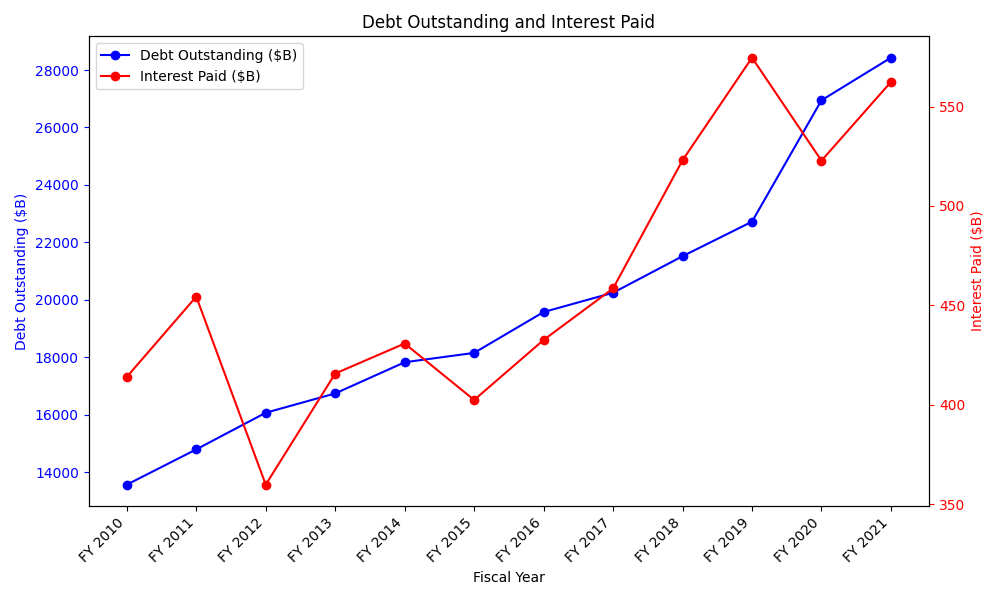
\includegraphics[scale=0.55]{img/debt_interest_paid.png}
      \caption{Debt Oustanding vs Interest Paid on debt.} 
      \label{fig:debt_interest_paid}
    \end{figure}

    We can break down national debt into three categories:

    \begin{enumerate}
      \item \textbf{Domestic debt}: Government (non-intragovernmental) accounts, mutual funds, depository institutions (banks, etc.), state \& local governments, pension funds, insurance companies.
      \item \textbf{Foriegn debt}: Foreign countries, national governments, international investors.
      \item \textbf{Intragovernmental Debt}: This is for the Social Security Tax Fund. When the government collects payroll taxes (the main source of income for OASDI), it invests them into U.S. treasury securities. This is weird because one governmental entity is buying bonds from another governmental entity, both under the same umbrella. However, these intragovernmental bonds are special because they are \textit{only} reserved for the trust funds, bought only with payroll taxes, and are not marketable. Thus, the OASDI fund is invested in T-bonds, isolated within the government, for a consistent return that is needed for social security benefits.
    \end{enumerate}

    \begin{figure}[H]
      \centering 
      % \includegraphics[scale=0.4]{img/}
      \caption{\href{https://ticdata.treasury.gov/Publish/mfh.txt}{\textit{Major Foreign Holders of Treasury Securities}}} 
      \label{fig:foreign_debt_holders}
    \end{figure}

    Some points to make:
    \begin{enumerate}
      \item Japan and China are the biggest creditors to the U.S. The low and negative bond yields in Japan make U.S. securities more attractive.
      \item China's large holdings is justified through its rapidly expanding economy.
    \end{enumerate}

    \subsubsection{Domestic Debt}

    \subsubsection{Foreign Debt}

    \subsubsection{Intragovernmental Debt}

    \subsubsection{Debt Ceilings}

      Clearly, just giving out money by selling debt is not a good idea. 
      \begin{enumerate}
        \item This would cause massive inflation. 
      \end{enumerate}

      \begin{definition}
        The \textbf{debt ceiling} is a legislative limit on the amount of national debt that can be incurred by the U.S. treasury, limiting how much money the federal government must pay on the debt they already borrowed. It applies to the gross debt, which includes debt in the hands of the public and in intra-government accounts. If the U.S. national debt levels bump up against the ceiling, the Treasury Department must resort to other "extraordinary" measures to pay government obligations and expenditures until the ceiling is raised again.
      \end{definition}

      In 1917, the debt ceiling was created during World War 1 to make the federal government fiscally responsible. Since the 1960s, the debt ceiling has been raised 76 times whenever the U.S. has approached that limit. There are debates on whether this ceiling actually keeps the government responsible, since it's been raised so many times. But if it hit the ceiling, the United States would not be able to cover its deficit since domestic and foreign income become choked off, leaving the U.S. with the option of debt monetization or other extraordinary measures.

      \begin{figure}[H]
        \begin{table}[H]
          \begin{tabular}{|lr|lr|}
          \hline
          Aug 93 & 4,900  & Feb 09 & 12,104 \\
          Mar 96 & 5,500  & Feb 10 & 14,294 \\
          Jun 02 & 6,400  & Jan 12 & 16,394 \\
          Mar 06 & 8,965  & Feb 13 & Suspd. \\
          Jun 08 & 10,615 & Feb 14 & Suspd. \\
          Oct 08 & 11,315 & Mar 17 & 19,847 \\
          &        & Sep 17 & Suspd. \\
          &        & Mar 19 & 22,030 \\
          \hline
          \end{tabular}
        \end{table}
        \caption{Historical debt ceiling levels in billions USD. Note that these figures are unadjusted for the time value of money, such as interest and inflation.} 
        \label{fig:debt_ceilings}
      \end{figure}
      
      Throughout history, there have been numerous \href{https://en.wikipedia.org/wiki/History_of_the_United_States_debt_ceiling#Number_of_requests_for_increase}{debt ceiling crises}. 

      \begin{example}[1995 Debt Ceiling Crisis]
        
      \end{example}

      \begin{example}[2011 Debt Ceiling Crisis]
        
      \end{example}

      \begin{example}[2013 Debt Ceiling Crisis]
        
      \end{example}

      \begin{example}[2021 Debt Ceiling Crisis]
        
      \end{example}

  \subsection{Debt Restructuring}

\end{document}
